%!TEX program = pdflatex
\documentclass[conference]{IEEEtran}

\usepackage{ifluatex}
\ifluatex
  \usepackage{fontspec}
  \usepackage{polyglossia} % babel replacement for use with fontspec
  \setdefaultlanguage[variant=american]{english}
  \selectlanguage[variant=american]{english}
\else
  \usepackage[utf8]{inputenc}
  \usepackage[T1]{fontenc}
  \usepackage[american]{babel}
  \usepackage{textcomp}
  %\DeclareUnicodeCharacter{20AC}{\euro{}}
  %\usepackage{eurosym}
\fi

\usepackage[acronym, nomain, nowarn]{glossaries}
\loadglsentries{acronyms}
\usepackage[hyphens]{url}
%\usepackage[pdfhighlight=/O, hidelinks, unicode=true]{hyperref}
\usepackage{mathtools}
\usepackage{fixmath}
\usepackage{algorithm2e}
%\usepackage{subcaption}
\usepackage{siunitx}
%\DeclareSIUnit{\EUR}{\text{\texteuro}} % gulps up subsequent symbols, commented out
\DeclareSIUnit\year{yrs}
\sisetup{load-configurations = abbreviations,binary-units, per-mode=symbol}
\usepackage{csquotes}
\usepackage{booktabs}
\usepackage{tabu}
\usepackage{rotating}
\makeglossaries
\usepackage[url=false,doi=false,backend=biber,style=ieee,isbn=false,sorting=none,minnames=1,maxnames=2]{biblatex}
\addbibresource{literature.bib}
\usepackage[inline]{enumitem}

\usepackage[np]{numprint}
\npstyleenglish

\usepackage[bordercolor=white]{todonotes}
\usepackage{balance}


\usepackage{cleveref}
\crefformat{footnote}{#2\footnotemark[#1]#3}

\usepackage{xspace}
\newcommand{\steam}{\textsc{Steam}\xspace}
\newcommand{\hltb}{\textsc{How Long To Beat}\xspace}
\newcommand{\metacritic}{\textsc{Metacritic}\xspace}
\newcommand{\gfnow}{\textsc{GeForce NOW}\xspace}
\newcommand{\gfnowpc}{\textsc{GeForce NOW} for \gls{PC}\xspace}
\newcommand{\psnow}{\textsc{PlayStation Now}\xspace}
\newcommand{\psnowpc}{\textsc{PlayStation Now} on \gls{PC}\xspace}
\newcommand{\liquid}{\textsc{LiquidSky}\xspace}


\begin{document}

\title{Subjective And Objective Assessment Of Video Game Context Factors}

%
%\author{\IEEEauthorblockN{Albert Rafetseder}
%\IEEEauthorblockA{NYU Tandon School Of Engineering, USA\\
%\texttt{albert.rafetseder@univie.ac.at}}
%\and
%\IEEEauthorblockN{Florian Metzger}
%\IEEEauthorblockA{Chair of Modeling of Adaptive Systems\\
%University of Duisburg-Essen, Germany\\
%\texttt{florian.metzger@uni-due.de}}
%\and
%\IEEEauthorblockN{Svenja Schröder}
%\IEEEauthorblockA{Universität Wien, Austria\\
%\texttt{svenja.schroeder@univie.ac.at}}
%}


\maketitle

%!TEX root = paper.tex
%%%%%%%%%%%%%%%%%%%%%%%%%%%%%%%%%%%%%%%%%%%%%%%%%%%%%%%%%%%%%%%%%%%%%%%%%%%%%%%

\newglossaryentry{cg}{name={cloud gaming},description={Gaming in the cloud}}


%\newacronym[description={\glslink{2g}{Second Generation}}]{2G}{2G}{Second Generation}
\newacronym{2G}{2G}{Second Generation}
\newacronym{3G}{3G}{Third Generation}
\newacronym{3GPP}{3GPP}{Third Generation Partnership Project}
\newacronym{AAA}{AAA}{Authentication, Authorization and Accounting}
\newacronym{AAC}{AAC}{Advanced Audio Coding}
\newacronym{ABI}{ABI}{Application Binary Interface}
\newacronym{AMBR}{AMBR}{Aggregate Maximum Bit-Rate}
\newacronym{ANOVA}{ANOVA}{Analysis of Variance}
\newacronym{API}{API}{Application Programming Interface}
\newacronym{APM}{APM}{Actions per Minute}
\newacronym{APN}{APN}{Access Point Name}
\newacronym{AQM}{AQM}{Active Queue Management}
\newacronym{ARQ}{ARQ}{Automatic Repeat Request}
\newacronym{ASN.1}{ASN.1}{Abstract Syntax Notation One}
\newacronym{ATM}{ATM}{Asynchronous Transfer Mode}
\newacronym{AU}{AU}{Access Unit}
\newacronym{AuC}{AuC}{Authentication Centre}
\newacronym{AVC}{AVC}{Advanced Video Coding}
\newacronym{BDP}{BDP}{Bandwidth-Delay Product}
\newacronym{BGP}{BGP}{Border Gateway Protocol}
\newacronym{BMC}{BMC}{Broadcast/Multicast Control}
\newacronym{BSC}{BSC}{Base Station Controller}
\newacronym{BSD}{BSD}{Berkeley Software Distribution}
\newacronym{BSS}{BSS}{Base Station Subsystem}
\newacronym{BTS}{BTS}{Base Transceiver Station}
\newacronym{CAMEL}{CAMEL}{Customised Applications for Mobile Networks Enhanced Logic}
\newacronym{CAPEX}{CAPEX}{CAPital EXpenditure}
\newacronym{CCG}{CCG}{Collectible Card Game}
\newacronym{CDF}{CDF}{Cumulative Distribution Function}
\newacronym{CDN}{CDN}{Content Distribution Network}
\newacronym{CDMA}{CDMA}{Code Division Multiple Access}
\newacronym{CELLDCH}{CELL\_DCH}{Dedicated Channel}
\newacronym{CELLFACH}{CELL\_FACH}{Forward Access Channel}
\newacronym{CELLPCH}{CELL\_PCH}{Cell Paging Channel}
\newacronym{CGN}{CGN}{Carrier-grade \acrshort{NAT}}
\newacronym{CI}{CI}{Continuity Index}
\newacronym{CN}{CN}{Core Network}
\newacronym{CPU}{CPU}{Central Processing Unit}
\newacronym{CS}{CS}{Circuit Switching}
\newacronym{CSG}{CSG}{Closed Subscriber Group}
\newacronym{CSS}{CSS}{Cascading Style Sheets}
\newacronym{DANE}{DANE}{DNS-Based Authentication of Named Entities}
\newacronym{DASH}{DASH}{Dynamic Adaptive Streaming over \acrshort{HTTP}}
\newacronym{DCCP}{DCCP}{Datagram Congestion Control Protocol}
\newacronym{DCE}{DCE}{Direct Code Execution}
\newacronym{DDoS}{DDoS}{Distributed \acrshort{DoS}}
\newacronym{DES}{DES}{Discrete Event Simulation}
\newacronym{DF}{DF}{Delay Factor}
\newacronym{DLEP}{DLEP}{Dynamic Link Exchange Protocol}
\newacronym{DLNA}{DLNA}{Digital Living Network Alliance}
\newacronym{DNS}{DNS}{Domain Name System}
\newacronym{DNSSEC}{DNSSEC}{\acrshort{DNS} Security Extensions}
\newacronym{DOCSIS}{DOCSIS}{Data Over Cable Service Interface Specification}
\newacronym{DoS}{DoS}{Denial of Service}
\newacronym{DPI}{DPI}{Deep Packet Inspection}
\newacronym{DRM}{DRM}{Digital Rights Management}
\newacronym{DSL}{DSL}{Digital Subscriber Line}
\newacronym{DTLS}{DTLS}{Datagram \acrshort{TLS}}
\newacronym{DTN}{DTN}{Delay-Tolerant Networking}
\newacronym{E2E}{E2E}{end-to-end}
\newacronym{ECDF}{ECDF}{Empirical \acrshort{CDF}}
\newacronym{ECM}{ECM}{EPS Connection Management}
\newacronym{ECN}{ECN}{Explicit Congestion Notification}
\newacronym{EDGE}{EDGE}{Enhanced Data Rates for \acrshort{GSM} Evolution}
\newacronym{EEG}{EEG}{Electroencephalography}
\newacronym{EIR}{EIR}{Equipment Identity Register}
\newacronym{EMM}{EMM}{Evolved Mobility Management}
\newacronym{eNB}{eNB}{Evolved Node B}
\newacronym{EPC}{EPC}{Evolved Packet Core}
\newacronym{EPS}{EPS}{Evolved Packet System}
\newacronym{ES}{ES}{Elementary Stream}
\newacronym{ETSI}{ETSI}{European Telecommunications Standards Institute}
\newacronym{E-UTRAN}{E-UTRAN}{Evolved \acrshort{UTRAN}}
\newacronym{FEC}{FEC}{Forward Error Correction}
\newacronym{fEMG}{fEMG}{Facial Electromyography}
\newacronym{FPS}{FPS}{First-Person Shooter}
\newacronym{FOSS}{FOSS}{Free and open-source software}
\newacronym{FSM}{FSM}{finite-state machine}
\newacronym{FTW}{FTW}{Telecommunications Research Center Vienna}
\newacronym{GERAN}{GERAN}{\acrshort{GSM}/\acrshort{EDGE} Radio Access Network}
\newacronym{GGSN}{GGSN}{Gateway \acrshort{GPRS} Support Node}
\newacronym{GMSC}{GMSC}{Gateway \acrshort{MSC}}
\newacronym{GPL}{GPL}{GNU General Public License}
\newacronym{GPLv3}{GPLv3}{\acrshort{GPL} version 3}
\newacronym{GPRS}{GPRS}{General Packet Radio System}
\newacronym{GPS}{GPS}{Global Positioning System}
\newacronym{GSM}{GSM}{Global System for Mobile Communications}
\newacronym{GSMA}{GSMA}{\acrshort{GSM} Association}
\newacronym{gtp}{GTP}{GPRS Tunneling Protocol}
\newacronym{GTP-C}{GTP-C}{\acrshort{gtp} Control}
\newacronym{GTP-U}{GTP-U}{\acrshort{gtp} User}
\newacronym{gtpv2}{GTPv2}{\acrshort{gtp} version 2}
\newacronym{GPU}{GPU}{Graphics Processing Unit}
\newacronym{GUI}{GUI}{Graphical User Interface}
\newacronym{HLR}{HLR}{Home Location Register}
\newacronym{HLS}{HLS}{HTTP Live Streaming}
\newacronym{HOL}{HOL}{Head-of-line}
\newacronym{HSDPA}{HSDPA}{High-Speed Downlink Packet Access}
\newacronym{HSPA}{HSPA}{High Speed Packet Access}
\newacronym{HSPA+}{HSPA+}{High Speed Packet Access Plus}
\newacronym{HSS}{HSS}{Home Subscriber Server}
\newacronym{HSUPA}{HSUPA}{High Speed Uplink Packet Access}
\newacronym{HTML}{HTML}{HyperText Markup Language}
\newacronym{HTTP}{HTTP}{HyperText Transfer Protocol}
\newacronym{HTTPS}{HTTPS}{\acrshort{HTTP} Secure}
\newacronym{IAB}{IAB}{Internet Architecture Board}
\newacronym{IAT}{IAT}{Inter Arrival Time}
\newacronym{ICE}{ICE}{Interactive Connectivity Establishment}
\newacronym{ICMP}{ICMP}{Internet Control Message Protocol}
\newacronym{IE}{IE}{Information Element}
\newacronym{IEC}{IEC}{International Electrotechnical Commission}
\newacronym{IEEE}{IEEE}{Institute of Electrical and Electronics Engineers}
\newacronym{IETF}{IETF}{Internet Engineering Task Force}
\newacronym{IGMP}{IGMP}{Internet Group Management Protocol}
\newacronym{IMAP}{IMAP}{Internet Message Access Protocol}
\newacronym{IMAPS}{IMAPS}{\acrshort{IMAP} Secure}
\newacronym{IMEI}{IMEI}{International Mobile Equipment Identity}
\newacronym{IMS}{IMS}{IP Multimedia Subsystem}
\newacronym{IMSI}{IMSI}{International Mobile Subscriber Identity}
\newacronym{IoE}{IoE}{Internet of Everything}
\newacronym{IoT}{IoT}{Internet of Things}
\newacronym{IP}{IP}{Internet Protocol}
\newacronym{IPC}{IPC}{Inter-Process Communication}
\newacronym{IPv4}{IPv4}{\acrshort{IP} version 4}
\newacronym{IPv6}{IPv6}{\acrshort{IP} version 6}
\newacronym{IPTV}{IPTV}{Internet Protocol television}
\newacronym{ISDN}{ISDN}{Integrated Services Digital Network}
\newacronym{ISO}{ISO}{International Organization for Standardization}
\newacronym{ISOC}{ISOC}{Internet Society}
\newacronym{ISP}{ISP}{Internet Service Provider}
\newacronym{ITU}{ITU}{International Telecommunication Union}
\newacronym{ITU-T}{ITU-T}{\acrshort{ITU} Telecommunication Standardization Sector}
\newacronym{JSON}{JSON}{JavaScript Object Notation}
\newacronym{KISS}{KISS}{``Keep it simple, stupid''}
\newacronym{LAN}{LAN}{Local Area Network}
\newacronym{LEDBAT}{LEDBAT}{Low Extra Delay Background Transport}
\newacronym{LGPLv3}{LGPLv3}{GNU Lesser General Public License version 3}
\newacronym{LISP}{LISP}{Locator/Identifier Separation Protocol}
\newacronym{LTE}{LTE}{Long Term Evolution}
\newacronym{M2M}{M2M}{Machine-to-Machine}
\newacronym{MAC}{MAC}{Media Access Control}
\newacronym{MANET}{MANET}{Mobile Ad Hoc Network}
\newacronym{MAP}{MAP}{Mobile Application Part}
\newacronym{MBMS}{MBMS}{Multimedia Broadcast Multicast Services}
\newacronym{MBR}{MBR}{Maximum Bitrate}
\newacronym{MDI}{MDI}{Media Delivery Index}
\newacronym{METAWIN}{METAWIN}{Measurement and Traffic Analysis in Wireless Networks}
\newacronym{MGW}{MGW}{Media Gateway}
\newacronym{MIME}{MIME}{Multipurpose Internet Mail Extensions}
\newacronym{MM}{MM}{Mobility Management}
\newacronym{MME}{MME}{Mobility Management Entity}
\newacronym{MMO}{MMO}{Massively Multiplayer Online}
\newacronym{MMS}{MMS}{Microsoft Media Server}
\newacronym{MOS}{MOS}{Mean Opinion Score}
\newacronym{MS}{MS}{Mobile Station}
\newacronym{MS-ID}{MS-ID}{Mobile Station Identifier}
\newacronym{MSC}{MSC}{Mobile Switching Center}
\newacronym{MSISDN}{MSISDN}{Mobile Subscriber Integrated Services Digital Network-Number}
\newacronym{MSE}{MSE}{Mean Squared Error}
\newacronym{MTC}{MTC}{Machine-Type Communications}
\newacronym{MTU}{MTU}{Maximum Transmission Unit}
\newacronym{NAS}{NAS}{Network-Attached Storage}
\newacronym{NAT}{NAT}{Network Address Translation}
\newacronym{NBAP}{NBAP}{Node B Application Part}
\newacronym{NFC}{NFC}{Near Field Communication}
\newacronym{NFV}{NFV}{Network Function Virtualization}
\newacronym{NSAPI}{NSAPI}{Network Service Access Point Identifier}
\newacronym{NSC}{NSC}{Network Simulation Cradle}
\newacronym{O3GM}{O3GM}{Open3G Map}
\newacronym{OMC}{OMC}{Operation and Maintenance Centre}
\newacronym{OPEX}{OPEX}{OPerational EXpenditure}
\newacronym{os}{OS}{Operating System}
\newacronym{OSI}{OSI}{Open Systems Interconnection}
\newacronym{OSPF}{OSPF}{Open Shortest Path First}
\newacronym{P2P}{P2P}{Peer-to-Peer}
\newacronym{PAN}{PAN}{Personal Area Network}
\newacronym{PC}{PC}{Personal Computer}
\newacronym{PCC}{PCC}{Policy and Charging Control}
\newacronym{PCO}{PCO}{Protocol Configuration Options}
\newacronym{PCEF}{PCEF}{Policy and Charging Enforcement Function}
\newacronym{PCRF}{PCRF}{Policy and Charging Rules Function}
\newacronym{PDCP}{PDCP}{Packet Data Convergence Protocol}
\newacronym{PDN}{PDN}{Public Data Network}
\newacronym{PDP}{PDP}{Packet Data Protocol}
\newacronym{PEVQ}{PEVQ}{Perceptual Evaluation of Video Quality}
\newacronym{PGW}{PGW}{Packet Gateway}
\newacronym{PI}{PI}{Pause Intensity}
\newacronym{PLMN}{PLMN}{Public Land Mobile Network}
\newacronym{PMIPv6}{PMIPv6}{Proxy Mobile \acrshort{IPv6}}
\newacronym{PMTU}{PMTU}{Path \acrshort{MTU}}
\newacronym{PON}{PON}{Passive Optical Network}
\newacronym{PPPoE}{PPPoE}{Point-to-Point Protocol over Ethernet}
\newacronym{PRNG}{PRNG}{Pseudorandom Number Generator}
\newacronym{PS}{PS}{Packet Switching}
\newacronym{PSNR}{PSNR}{Peak Signal-to-Noise Ratio}
\newacronym{QoE}{QoE}{Quality of Experience}
\newacronym{QoS}{QoS}{Quality of Service}
\newacronym{QUIC}{QUIC}{Quick UDP Internet Connections}
\newacronym{RAB}{RAB}{Radio Access Bearer}
\newacronym{RAN}{RAN}{Radio Access Network}
\newacronym{RANAP}{RANAP}{Radio Access Network Application Part}
\newacronym{RAI}{RAI}{Routeing Area Identity}
\newacronym{RBI}{RBI}{Reporting Body Identifier}
\newacronym{RAT}{RAT}{Radio Access Technology}
\newacronym{REST}{REST}{Representational State Transfer}
\newacronym{RFC}{RFC}{Request for Comments}
\newacronym{RIP}{RIP}{Routing Information Protocol}
\newacronym{RLC}{RLC}{Radio Link Control}
\newacronym{RNC}{RNC}{Radio Network Controller}
\newacronym{RPC}{RPC}{Remote Procedure Call}
\newacronym{RPG}{RPG}{Role-Playing Game}
\newacronym{RRC}{RRC}{Radio Resource Control}
\newacronym{RSS}{RSS}{Rich Site Summary}
\newacronym{rtcp}{RTCP}{\acrshort{rtp} Control Protocol}
\newacronym{RTMP}{RTMP}{Real Time Messaging Protocol}
\newacronym{rtp}{RTP}{Real-time Transport Protocol}
\newacronym{RTS}{RTS}{Real-time Strategy game}
\newacronym{RTSP}{RTSP}{Real Time Streaming Protocol}
\newacronym{RTT}{RTT}{Round-Trip Time}
\newacronym{RV}{RV}{Random Variable}
\newacronym{S1AP}{S1AP}{S1 Application Protocol}
\newacronym{SAE}{SAE}{System Architecture Evolution}
\newacronym{SAP}{SAP}{Session Announcement Protocol}
\newacronym{osiSAP}{SAP}{Service Access Point}
\newacronym{SCCP}{SCCP}{Signalling Connection Control Part}
\newacronym{SCTP}{SCTP}{Stream Control Transmission Protocol}
\newacronym{SDN}{SDN}{Software Defined Networking}
\newacronym{SMTP}{SMTP}{Simple Mail Transfer Protocol}
\newacronym{SMTPS}{SMTPS}{\acrshort{SMTP} Secure}
\newacronym{SDP}{SDP}{Session Description Protocol}
\newacronym{SDR}{SDR}{Software Defined Radio}
\newacronym{SGSN}{SGSN}{Serving \acrshort{GPRS} Support Node}
\newacronym{SGW}{SGW}{Serving Gateway}
\newacronym{SIM}{SIM}{Subscriber Identity Module}
\newacronym{SIP}{SIP}{Session Initiation Protocol}
\newacronym{SQL}{SQL}{Structured Query Language}
\newacronym{SS7}{SS7}{Signalling System No. 7}
\newacronym{SSD}{SSD}{Solid State Disk}
\newacronym{SSIM}{SSIM}{Structural SIMilarity}
\newacronym{STUN}{STUN}{Session Traversal Utilities for \acrshort{NAT}}
\newacronym{SV}{SV}{Software Version}
\newacronym{SVC}{SVC}{Scalable Video Coding}
\newacronym{POTS}{POTS}{Plain Old Telephone Service}
\newacronym{PSTN}{PSTN}{Public Switched Telephone Network}
\newacronym{TAC}{TAC}{Type Allocation Code}
\newacronym{TCAP}{TCAP}{Transaction Capabilities Application Part}
\newacronym{TCP}{TCP}{Transmission Control Protocol}
\newacronym{TEID}{TEID}{Tunnel Endpoint Identifier}
\newacronym{TFT}{TFT}{Traffic Flow Template}
\newacronym{TLS}{TLS}{Transport Layer Security}
\newacronym{TS}{TS}{Technical Specification}
\newacronym{TTI}{TTI}{Transmission Time Interval}
\newacronym{UDP}{UDP}{User Datagram Protocol}
\newacronym{UE}{UE}{User Equipment}
\newacronym{UMTS}{UMTS}{Universal Mobile Telecommunications System}
\newacronym{UPnP}{UPnP}{Universal Plug and Play}
\newacronym{URA}{URA}{\acrshort{UTRAN} Registration Area}
\newacronym{URAPCH}{URA\_PCH}{\acrshort{URA} Paging Channel}
\newacronym{URL}{URL}{Uniform Resource Locator}
\newacronym{USIM}{USIM}{Universal Subscriber Identity Module}
\newacronym{uTP}{$\mu$TP}{Micro Transport Protocol}
\newacronym{UTRAN}{UTRAN}{\acrshort{UMTS} Terrestrial Radio Access Network}
\newacronym{VANET}{VANET}{Vehicular Ad Hoc Network}
\newacronym{VDSL}{VDSL}{Very-high-bit-rate Digital Subscriber Line}
\newacronym{VB}{VB}{Virtual Buffer}
\newacronym{VM}{VM}{Virtual Machine}
\newacronym{VMM}{VMM}{Virtual Machine Manager}
\newacronym{VoD}{VoD}{Video on Demand}
\newacronym{VoIP}{VoIP}{Voice over \acrshort{IP}}
\newacronym{VQEG}{VQEG}{Video Quality Experts Group}
\newacronym{W3C}{W3C}{World Wide Web Consortium}
\newacronym{WebRTC}{WebRTC}{Web Real-Time Communication}
\newacronym{WMSP}{WMSP}{Windows Media \acrshort{HTTP} Streaming Protocol}
\newacronym{XML}{XML}{Extensible Markup Language}
\newacronym{XMPP}{XMPP}{Extensible Messaging and Presence Protocol}

%!TEX root = paper.tex
%%%%%%%%%%%%%%%%%%%%%%%%%%%%%%%%%%%%%%%%%%%%%%%%%%%%%%%%%%%%%%%%%%%%%%%%%%%%%%%%
\begin{abstract}

%stagnate in terms of commercial success. 
In recent years, cloud gaming has become a popular research topic, and the list of its supposed benefits is long. However, cloud gaming platforms are still waiting for the commercial breakthrough. This might be caused by the pricing models and product offerings by existing ``à la carte'' platforms. This paper aims at investigating the costs and benefits of both platform types through a twofold approach. We first take on the perspective of the customers, and investigate several cloud gaming platforms and their pricing models in comparison to the costs of ``à la carte'' platforms. Then, we explore engagement metrics in order to assess the enjoyment of playing the offered games. Lastly, coming from the perspective of the service providers, we aim to give reasons for the problematic nature of operating a large-scale cloud gaming service while maintaining high \acrshort{QoE} values. Our analysis provides initial, yet still comprehensive reasons and models for the prospects of cloud gaming in a highly competitive market.

\end{abstract}

%!TEX root = paper.tex
%%%%%%%%%%%%%%%%%%%%%%%%%%%%%%%%%%%%%%%%%%%%%%%%%%%%%%%%%%%%%%%%%%%%%%%%
%%%%%%%

\todo[inline,color=red!10]{Other title could be: The Prospects of Cloud 
Gaming: Do ... }

\section{Introduction}

Cloud gaming has become quite a popular research topic in recent years. 
Much of this research is aimed at comparing the experienced 
quality of cloud gaming to that of conventional gaming approaches, with 
the results
% Albert: even in terms of cost effectiveness, potential choice of 
% games, lower demands on required end user hardware
% (AKA the usual cloud gaming selling points)?
generally in favor of conventional gaming, but only by a 
tiny margin. Some publications even praise the method and attest high 
\gls{QoE} values.

So, if there are only negligible quality drawbacks --- according to the 
literature --- what about the commercial success of cloud gaming? In 
theory, there could be large economic benefits for users that should 
foster a quick adaptation of such services. 
However, quite a few commercial services have already come and gone, 
with a rather high rate of fluctuation. For example, one of the most 
prominent services in the past, \textsc{OnLive}, shut down and was forced to 
sell off its remaining assets.

All cloud gaming services, current as well 
as past, come with some subtle differences in their service, including 
the technical aspects, the selection of games, and the pricing 
model.
Yet, differentiation has not helped to generate much more public 
interest either. 
This might be attributed to a circumstance that is easily  
overlooked when evaluating cloud gaming services: the strong 
competition with other non-cloud gaming platforms, such as the 
individual console platforms or the large market for PC games --- with the 
Steam\footnote{\url{http://store.steampowered.com/}} platform as one of 
its strongest contenders. The move to digital distribution has made the 
PC platform quite popular, and PC games pricing has become 
much more dynamic and affordable in the process.

On the surface, current Cloud Gaming services attempt to a adopt a 
\textit{fixed fee subscription} model over the traditional 
\textit{à la carte} model. 
This move proved to be hugely successful for other types of media, be 
it for example \textsc{Netflix} for movies and shows or 
\textsc{Spotify} for music. However, these two types of services seem 
to offer much more content at a comparable or even lower price point 
than Cloud Gaming services do. Additionally, the technical requirements 
to maintain a quality level on par with that of locally run games are 
also rather demanding.

The two main questions that this work aims to tackle are thus: 
\textit{``Can Cloud Gaming be attractive for users in today's highly 
competitive market?''} and \textit{``Can you operate a Cloud Gaming 
service with acceptable margins while maintaining acceptable quality 
levels?''}. Both questions are strongly intertwined as in order to make 
such services attractive one would have to offer sufficient quality and 
quantity of games with a competitive pricing while not operating at a 
loss. In practice one could actually simplify both questions quite 
easily to one: \textit{``Can you compete with the PC gaming and Steam 
ecosystem (in terms of quality, prices, and variety)?''}

In order to answer these questions, this paper looks at the perspective 
of users and service provider in separate and provides arguments backed 
by data and simple models. To investigate the customer's perspective we 
employ user domain-specific user engagement metrics --- amongst others 
review scores as well as the length and playtimes of games --- to 
compare various services --- Cloud Gaming as well as conventional --- 
to each other. Additionally, using this data some simple budget models 
are set up to compare what (in terms of the number and quality of 
games) for a certain amount of money. We find that in the investigated 
cases the Cloud Gaming services' offer is very limited yet still 
charges relatively high prices, thus limiting the attractiveness for 
users in comparison to alternative services.

Due to the limited amount of freely available data on operating a Cloud 
Gaming service, the perspective of the Cloud Gaming operator is 
investigated by setting up efficiency models centered around the 
overbooking rate. These initial figures highlight the problematic 
nature of Cloud Gaming in terms of scaling and cost efficiency. When 
compared to other cloud services, that achieve high values of cost 
efficiency and capacity utilization, we believe that Cloud Gaming 
platforms will be much more peak-oriented and can thus achieve much 
lower values of server utilization. The end-to-end lag requirements of 
games demand a server placement in the vicinity of the user and thus 
eliminate most multiplexing gains that a centralized data center can 
garner over the course of a day. Additionally, games require dedicated 
hardware support, which is of no much use to most other cloud use 
cases, diminishing the potential of cross-service reuse.

These initial insights do not shed a good light on the commercial 
future of Cloud Gaming services in general. Apart from achieving major 
cost reductions, while maintaining or better even improving streaming 
quality, the future of Cloud Gaming might be bleak. But there still 
might be some niches to place a Cloud Gaming service where the 
competition is less strong. We plan to take a deeper look at all these 
aspects and provide more detailed models in the future.

~\\
This paper is structured as follows. Sec.~\ref{sec:relatedwork} 
provides a brief overview of the related work. Afterwards, 
Sec.~\ref{sec:background} explains all the necessary terms and 
technical details to understand the topic. The main part of this work 
encompass Sections \ref{sec:engagement} and 
\ref{sec:suppliermodelling}, which conduct the dual-perspective 
investigation of the Cloud Gaming providers' and their competitions' 
business models and engagement from the angle of the user and the 
platform operator respectively. The paper concludes in 
Sec.~\ref{sec:conclusion} with some remarks and an outlook.

%%%%%%%%%%%%
% \subsection{Fragestellungen}

% \begin{itemize}
% 	\item Kostenmodell für Cloud Gaming Provider?
% 	\item Attraktivität für “Core Gamer”?
% 	\item Wieviel ist eine NutzerIn bereit für einen Streaming 
Service mit einem bestimmten Spieleangebot und einer bestimmten 
Streaming- Qualität (Video-Qualität, Latenz, Grafikeinstellungen des 
Spiels) zu zahlen?
% 	\item Can they be competitive against other gaming platforms, 
both from provider as well as customer perspective
% 			Most challenging: can it beat the Steam price 
model and quality/number of games? (plus bundle providers and sales)
% \end{itemize}
% Netflix-Analogie? 
%!TEX root = paper.tex
%%%%%%%%%%%%%%%%%%%%%%%%%%%%%%%%%%%%%%%%%%%%%%%%%%%%%%%%%%%%%%%%%%%%%%%%%%%%%%%
\section{Related Work}


%%%%%%%%%%%%%%%%%%%%%%%%%%%%%%%%%%%%%%%%%%%%%%%%%%%%%%%%%%%%%%%%%%%%%%%%%%%%%%%
\section{Cost of Cloud Gaming}

``Mobile Cloud Gaming: Issues and Challenges'' \cite{Soliman2013}
short overview of some possible issues

``Will Mobile Cloud Gaming Work? Findings on Latency, Energy, and Cost'' \cite{Lampe:2013:MCG:2514943.2515398}
client-side costs (monetary, energy, latency) of mobile devices; however underestimates energy costs in comparison to local gaming, display is the biggest factor, which is not factored in (this factor is also the same in local as well as cloud gaming); the monetary cost factor also underestimates the contractual situation in countries like Germany
And despite all this, it still finds mobile cloud gaming rather unfeasible (except in WiFi)

``Where Did My Battery Go? Quantifying the Energy Consumption of Cloud Gaming'' \cite{6924295}
Similar notion as previous paper, more in-depth, focus only on energy costs
test impl of local running game artificially increases cpu/gpu load
especially for low load games only marginal energy savings for cloud approach (~12\%)
even best case (and unrealistically high load) only 38\% energy savings
considering all the other drawbacks that cloud streaming incurs, this might not be enough

``Measuring the Client Performance and Energy Consumption in Mobile Cloud Gaming'' \cite{Huang:2014:MCP:2755535.2755542}
Similar findings, only 30\% energy savings


``Cloud gaming: a green solution to massive multiplayer online games'' \cite{6882299}
(TODO: need to read the full text yet)
Argues that removing computation intense tasks from (mobile) user devices leads to overall energy savings


Also approaches that select (and cost-optimize the selection of) data-centers might not be applicable due to the stringent latency and BW requirements and the need for dedicated hardware (GPUs) and the statefulness of gaming, e.g.
``QoS-Aware, Cost-Efficient Selection of Cloud Data Centers'' \cite{6740249}
``Cost-efficient Capacitation of Cloud Data Centers for QoS-aware Multimedia Service Provision.'' \cite{hans2014cost} optimization to geographically clustered users
``Placing Virtual Machines to Optimize Cloud Gaming Experience'' \cite{6853364}
latter paper includes many server cost optimization parameters, that might be worth looking at

Another optimization TODO: read fulltext
``QoS-Aware Revenue-Cost Optimization for Latency-Sensitive Services in IaaS Clouds'' \cite{6365107}

%%%%%%%%%%%%%%%%%%%%%%%%%%%%%%%%%%%%%%%%%%%%%%%%%%%%%%%%%%%%%%%%%%%%%%%%%%%%%%%
\section{Cloud Gaming in General}


%%%%%%%%%%%%%%%%%%%%%%%%%%%%%%%%%%%%%%%%%%%%%%%%%%%%%%%%%%%%%%%%%%%%%%%%%%%%%%%
\section{QoS/QoE of Gaming in General}

``On the Impact of Delay on Real-time Multiplayer Games'' \cite{Pantel:2002:IDR:507670.507674}

``The Effects of Loss and Latency on User Performance in Unreal Tournament 2003'' \cite{Beigbeder:2004:ELL:1016540.1016556}

``An experimental estimation of latency sensitivity in multiplayer Quake 3'' \cite{1266180}

``QoE Assessment of Interactivity and Fairness in First Person Shooting with Group Synchronization Control'' \cite{Ida:2010:QAI:1944796.1944806}

``Assessing the Impact of Game Type, Display Size and Network Delay on Mobile Gaming QoE'' \cite{beyer2014typedisplaydelayimpact}

``Latency and Player Actions in Online Games'' \cite{Claypool:2006:LPA:1167838.1167860}

%%%%%%%%%%%%
\subsection{Models}
``A Comprehensive End-to-End Lag Model for Online and Cloud Video Gaming'' \cite{metzger16lagmodel}


%%%%%%%%%%%%
\subsection{Measurements and Methods}

``A Method For Feedback Delay Measurement Using a Low-cost Arduino Microcontroller'' \cite{beyermethod}

``Towards a New {ITU-T} Recommendation for Subjective Methods Evaluating Gaming {QoE}'' \cite{mollertowards}

``Effect of Network Quality on Player Departure Behavior in Online Games'' \cite{4591393}

``An Empirical Study of Cloud Gaming'' \cite{Manzano:2012:ESC:2501560.2501582}

%%%%%%%%%%%%
\subsection{Studies}

``How Sensitive Are Online Gamers to Network Quality?'' \cite{Chen:2006:SOG:1167838.1167859}

``A Measurement Study Regarding Quality of Service and Its Impact on Multiplayer Online Games'' \cite{Bredel:2010:MSR:1944796.1944797}

``Empirical study of subjective quality for Massive Multiplayer Games'' \cite{4604397}



%%%%%%%%%%%%%%%%%%%%%%%%%%%%%%%%%%%%%%%%%%%%%%%%%%%%%%%%%%%%%%%%%%%%%%%%%%%%%%%
\section{QoS/QoE of Cloud Gaming}



``Modeling and Characterizing User Experience in a Cloud Server Based Mobile Gaming Approach'' (Shaoxuan Wang, Sujit Dey): http://esdat.ucsd.edu/projects/gaming/papers/globecom09.pdf

``The Impact of Video Encoding Parameters and Game Type on QoE for Cloud Gaming: a Case Study using the Steam Platform'' \cite{slivarimpact}

``On frame rate and player performance in first person shooter games'' \cite{claypool2007}


%%%%%%%%%%%%
\subsection{Measurements and Methods}
``Using Electroencephalography and Subjective Self-Assessment to Measure the Influence of Quality Variations in Cloud Gaming'' \cite{beyerusing}

``Cloud gaming: architecture and performance'' \cite{6574660}

``Measuring the Latency of Cloud Gaming Systems'' \cite{Chen:2011:MLC:2072298.2071991}

``On the Quality of Service of Cloud Gaming Systems'' \cite{6670099}

``The Brewing Storm in Cloud Gaming: A Measurement Study on Cloud to End-user Latency'' \cite{Choy:2012:BSC:2501560.2501563}

%%%%%%%%%%%%
\subsection{Subjective Studies}

``Gaming in the clouds: QoE and the users’ perspective'' \cite{Jarschel20132883}

``Are all games equally cloud-gaming-friendly? An electromyographic approach'' \cite{6404025}

``Subjective Evaluation of Latency and Packet Loss in a Cloud-Based Game'' \cite{6614351}

``An Evaluation of {QoE} in Cloud Gaming Based on Subjective Tests'' \cite{5976180}

%%%%%%%%%%%%
\subsection{QoE Adaptations}

video rate adaptations
``Addressing Response Time and Video Quality in Remote Server Based Internet Mobile Gaming'' \cite{5506572}

``Adaptive Mobile Cloud Computing to Enable Rich Mobile Multimedia Applications'' \cite{6413270}




%%%%%%%%%%%%%%%%%%%%%%%%%%%%%%%%%%%%%%%%%%%%%%%%%%%%%%%%%%%%%%%%%%%%%%%%%%%%%%%
\section{Other}


High frame rates:
``The Application of Sampling Theory to Television Frame Rate Requirements''
\url{http://www.bbc.co.uk/rd/publications/whitepaper282}
``High Frame-Rate Television''
\url{http://www.bbc.co.uk/rd/publications/whitepaper169}
``Higher Frame rates for more Immersive Video and Television''
\url{http://www.bbc.co.uk/rd/publications/whitepaper209}


Fundamental findings on framerates
``Experimentelle Studien über das Sehen von Bewegung'' \cite{wertheimer1912experimentelle}

VR:
``How Do New Visual Immersive Systems Influence Gaming QoE?'' \cite{7148110}


Hybrid Cloud/Local
``Kahawai: High-Quality Mobile Gaming Using GPU Offload'' \cite{Cuervo:2015:KHM:2742647.2742657}


Speculative Rendering of Future Frames
``Outatime: Using Speculation to Enable Low-Latency Continuous Interaction for Mobile Cloud Gaming'' \cite{Lee:2015:OUS:2742647.2742656}

``Security issues in online games'' \cite{doi:10.1108/02640470210424455}




%!TEX root = paper.tex
%%%%%%%%%%%%%%%%%%%%%%%%%%%%%%%%%%%%%%%%%%%%%%%%%%%%%%%%%%%%%%%%%%%%%%%%%%%%%%%%
\section{Background}



%%%%%%%%%%%%%%%%%%%%%%%%%%%%%%%%%%%%%%%%%%%%%%%%%%%%%%%%%%%%%%%%%%%%%%%%%%%%%%%%
\subsection{Service Costs of Gaming Platforms}

Price Models of:

\paragraph{Steam and PC in General}

\paragraph{Consoles}

\paragraph{Historical Example: OnLinve}


\paragraph{Geforce Now}
\url{http://shield.nvidia.com/game-streaming-with-geforce-now}
Kosten

\$7.99/mo + 200\$/€++ Hardware

Started in parts of Europe in Q4/2015

Spieleangebot

\$x Spiele im Paket

 + weitere/neuere zusätzlich mit Einmalbetrag

Leistung
Bandbreite? 

\paragraph{Playstation Now}
Streaming von PS3 Spielen auf PS4 und andere Sony-Geräte (als Rückwärtskompatibiliätslösung)
Kosten

(US/UK only?) Deuschlandbeta seit ~Q4/2015

\$ /mo + 330\$/€ (PS4) oder Sony TV + Controller
Extrakosten/Tagesleihgebühren für bestimmte ``bessere'' Spiele




%%%%%%%%%%%%%%%%%%%%%%%%%%%%%%%%%%%%%%%%%%%%%%%%%%%%%%%%%%%%%%%%%%%%%%%%%%%%%%%%
\subsection{Platform Provider Costs}
Backend/Service Requirements and Demands

%%%%%%%%%%%%
\subsubsection{CAPEX}

\begin{itemize}
	\item Regionale Data Center
	\item Gaming Server (GPU-Enabled)
	\item Entwicklungskosten für Software-Plattform(?)
\end{itemize}

\paragraph{Hardware}

\url{https://www.nvidia.com/object/cloud-gaming-gpu-boards.html}
\url{https://www.nvidia.com/object/grid-technology.html}


%%%%%%%%%%%%
\subsubsection{OPEX}

\paragraph{Verkehrsvolumen}

\begin{itemize}
	\item Internetanbindung?
	\item Caching of basic resources is probably not applicable?
\end{itemize}

\paragraph{Serverlaufzeiten}

\begin{itemize}
	\item Energie
	\item Verschleiß
	\item Wartungs- und Betriebspersonal oder Anmietung
	\item Frage: Rechnet sich Anmietung von Ressourcen bei großen generischen Rechenzentren? Annahme nein, da man selbst ein großer Anbieter wäre u. die Margin wegfallen. Auf der anderen Seite gibt es Hardware die für Games im Serverbereich besser skalieren? Wenn ja, kann umso mehr kein generischer Anbieter die Lösung sein
\end{itemize}

\paragraph{Spiele-Lizenzen und -Adaptionskosten (?)}
Modelannahme: Kosten pro Nutzung (realistisch eher in Blöcken verrechnet)





%%%%%%%%%%%%%%%%%%%%%%%%%%%%%%%%%%%%%%%%%%%%%%%%%%%%%%%%%%%%%%%%%%%%%%%%%%%%%%%%
\subsection{Data}

The leading question for the user side of the cost-benefit analysis is: ``How can we properly estimate the value a user gets from a specific service?'' with an additional question of ``What is the definition of value in this context?''

Simply counting the number of games one gets for a specific amount of money may be the easiest value metric but may also fall short. Therefore, this paper evaluates further approaches that also take game lengths and press review scores into account.

In order to achieve this, data had to be collected from various sources and merged into a consistent data base. All the scraping and merging code as well as the data itself can be found in the repositories at TODO to be verified by third parties. The following sections describe the individual data sources.

%%%%%%%%%%%%
\subsubsection{Steam API + SteamSpy Datensätze+Graphen}

Steam Sales:
Large seasonal sales (christmas, summer, lunar new year, halloween, fall, spring, ...) of many/most games on the platform usually rebates of 50\% and up.
Weekly sales
Daily sales
Weekend sales
Free weekends



\url{https://github.com/mas-ude/steam-data-stats} Steam + SteamSpy REST API Datensammler + ein paar Graphplotter (und eher ergebnislose Clustering-Versuche); für sinnvolle Analsyen müsste man dazu aber viel häufiger Datensätze generieren. Beispielausgaben:

CDF der Preise auf Steam (Juli ‘15) \ref{fig:steam-prices}

\begin{figure}[!t]
	\centering
	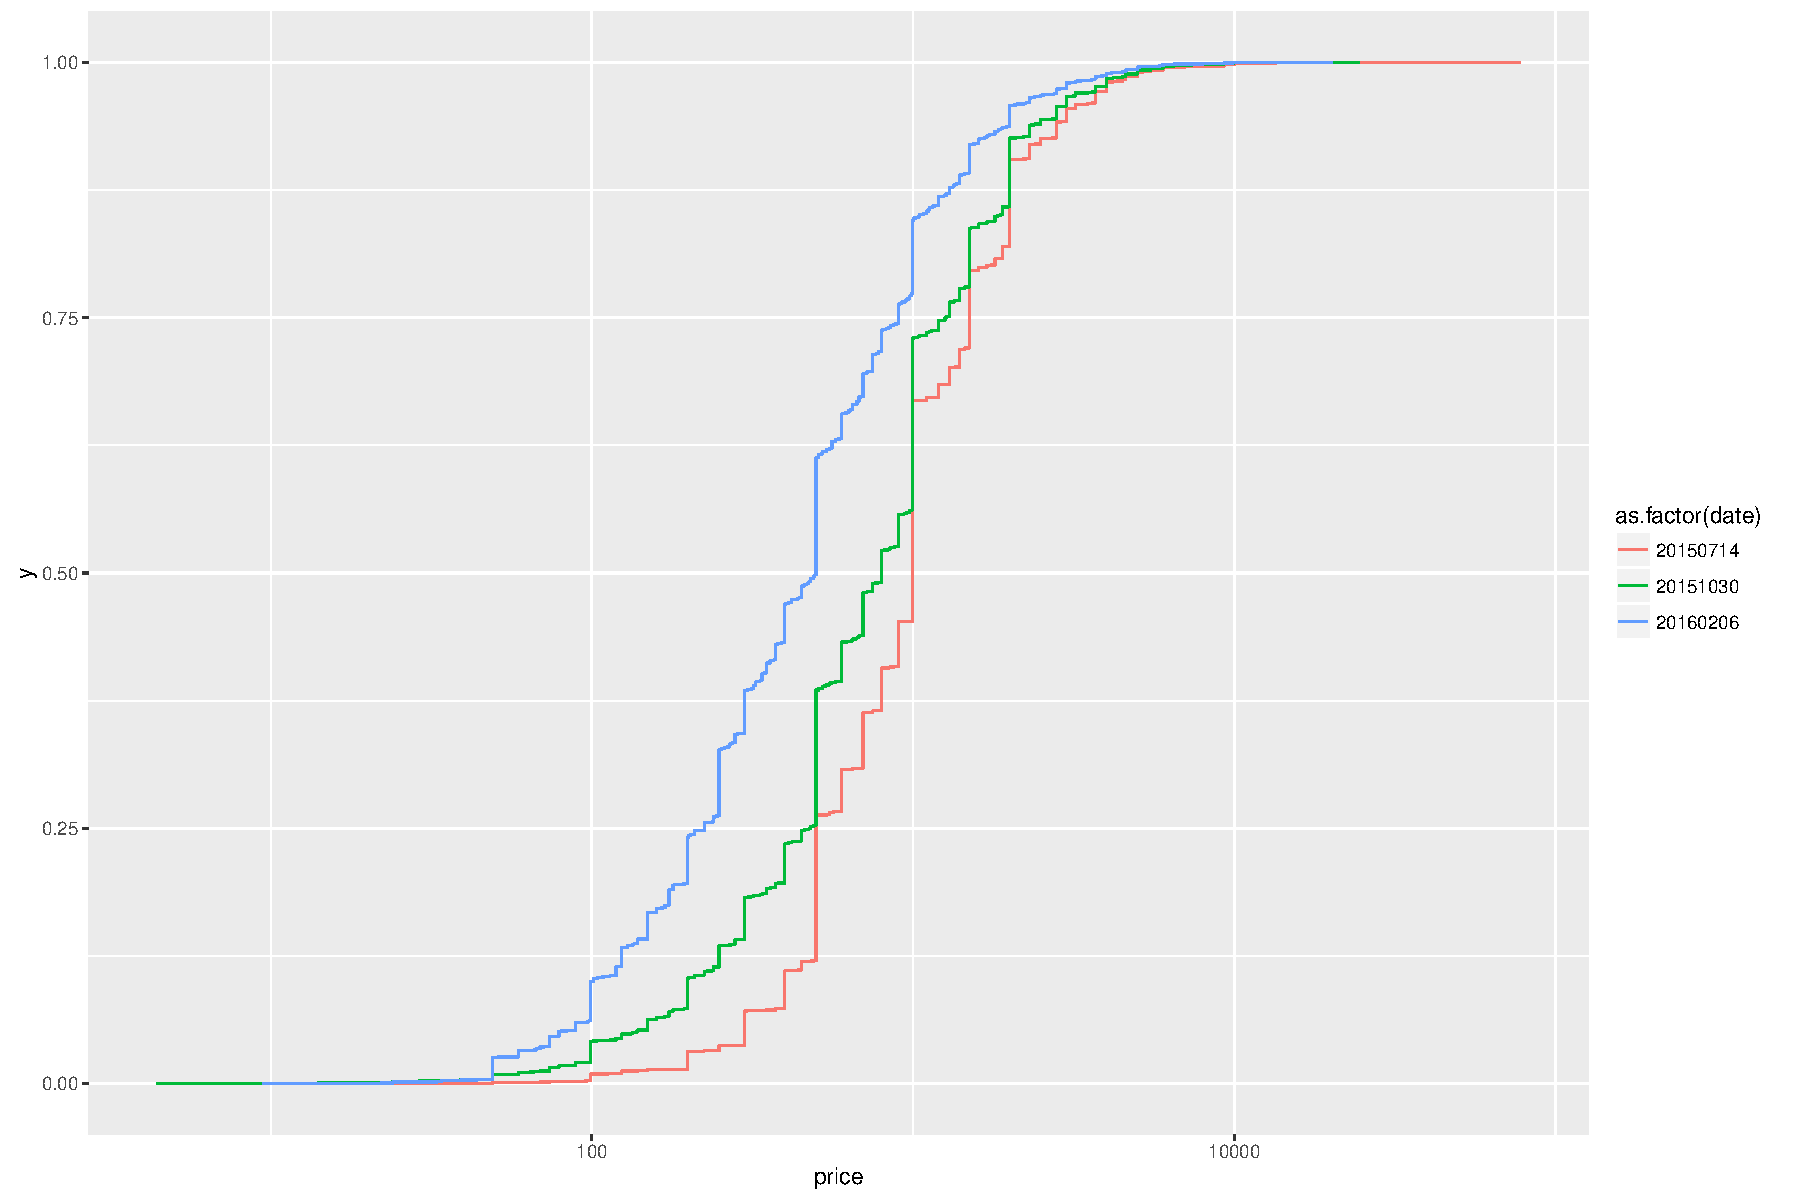
\includegraphics[width=1.0\columnwidth]{images/steam-prices.pdf}
	\caption{CDF of games on the steam platform at two distinct dates.}
\label{fig:steam-prices}
\end{figure}

Violinenplot der durchschnittlichen Spielzeit aufgeteilt auf unterschiedliche Preiskategorien. \ref{fig:steam-cost-vs-playtime-violin}

\begin{figure}[!t]
	\centering
	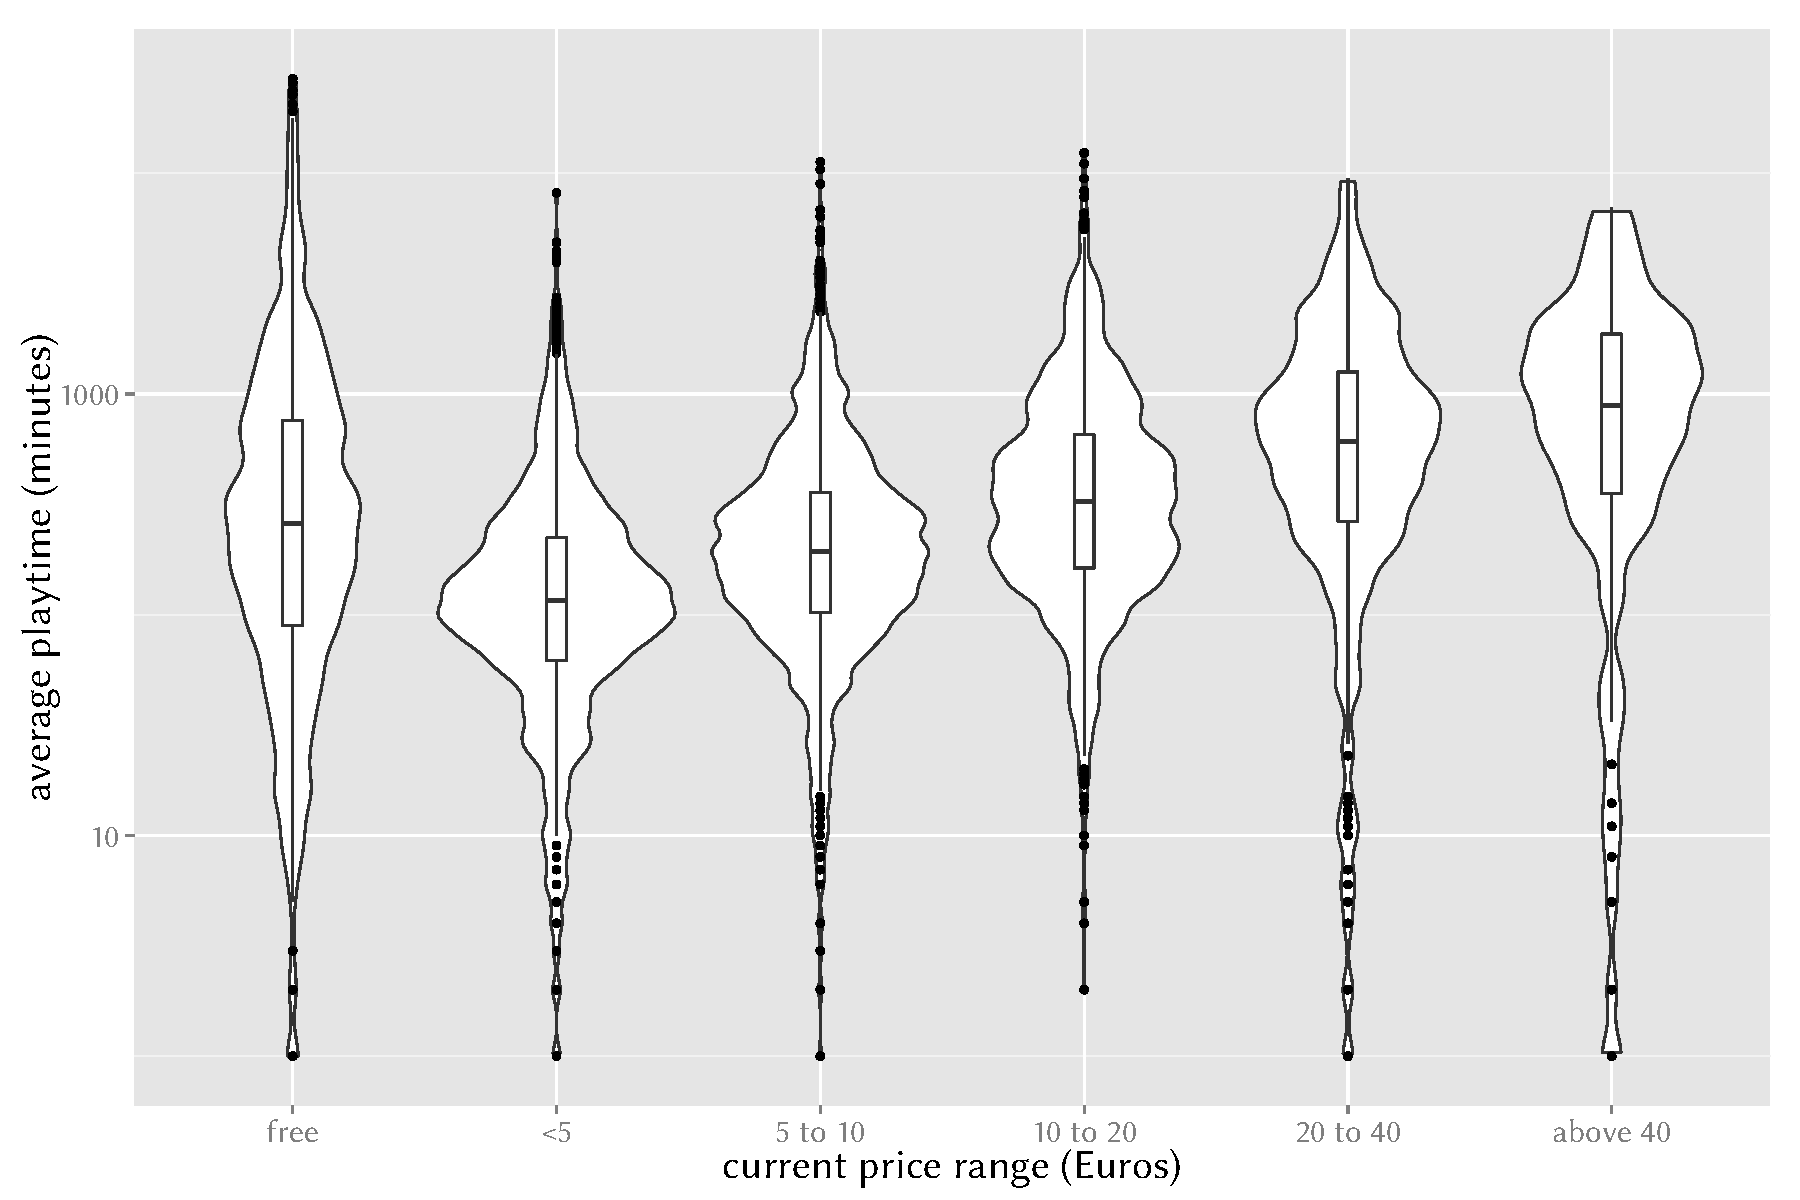
\includegraphics[width=1.0\columnwidth]{images/steam-cost-vs-playtime.pdf}
	\caption{Violin plot of the average playtime (as recorded by SteamSpy) of games categorized by their prices.}
\label{fig:steam-cost-vs-playtime-violin}
\end{figure}

%%%%%%%%%%%%
\subsubsection{HowLongToBeat Data}

Data scraped from \url{howlongtobeat.com}. This site allows for manual reporting of playthrough times of games on any platform. Times are separated into different play styles (e.g. ``main story'', ``completionist'') and only an aggregated time is shown. For this analysis only the average playtime of all play styles is taken into account.
It should however be stressed again, that this is a self-reporting site without strong validity checks. This has to be considered when contemplating the accuracy and validity of the data.

\begin{figure}[!t]
	\centering
	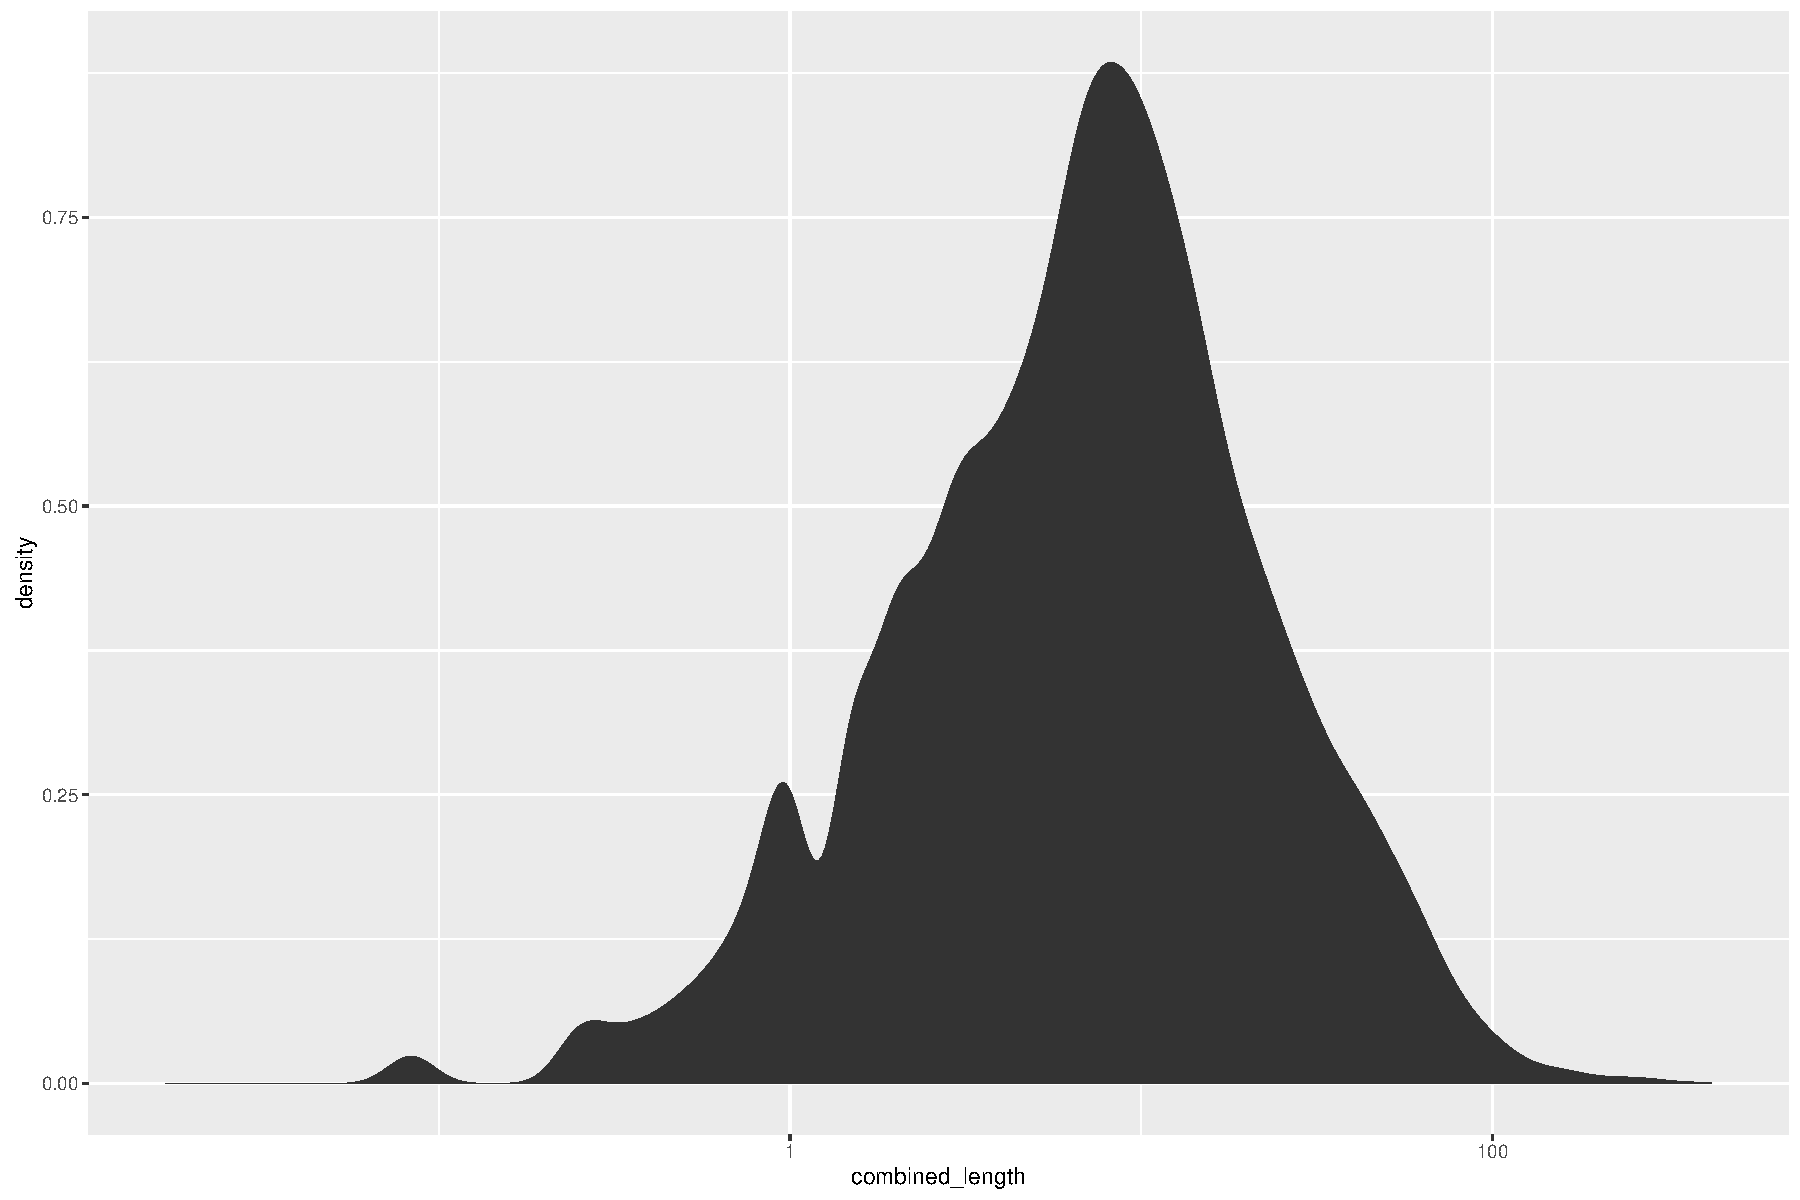
\includegraphics[width=1.0\columnwidth]{images/gamelengths-density.pdf}
	\caption{Density plot of the average game lengths over all play styles.}
\label{fig:gamelengths-density}
\end{figure}

Nonetheless, the distribution of game lengths from this set can still be worth to look at in the context of putting value to games for consumers of different platforms. As seen in Figure~\ref{fig:gamelengths-density} the play lengths vary greatly, with the median at \SI{7.5}{\hour} and a long tail of long play times reaching \SI{420}{\hour}.


%%%%%%%%%%%%
\subsubsection{Metacritic Data}

Game lengths can not only serve as an indicator of the amount of content a game has to offer, but can also serve as an engagement metric to estimate a user's amount of satisfaction. More fitting engagement metrics could also be employed.

% TODO: include or compare with data from opencritic.com as soon as their API is public/usable

\begin{figure}[!t]
	\centering
	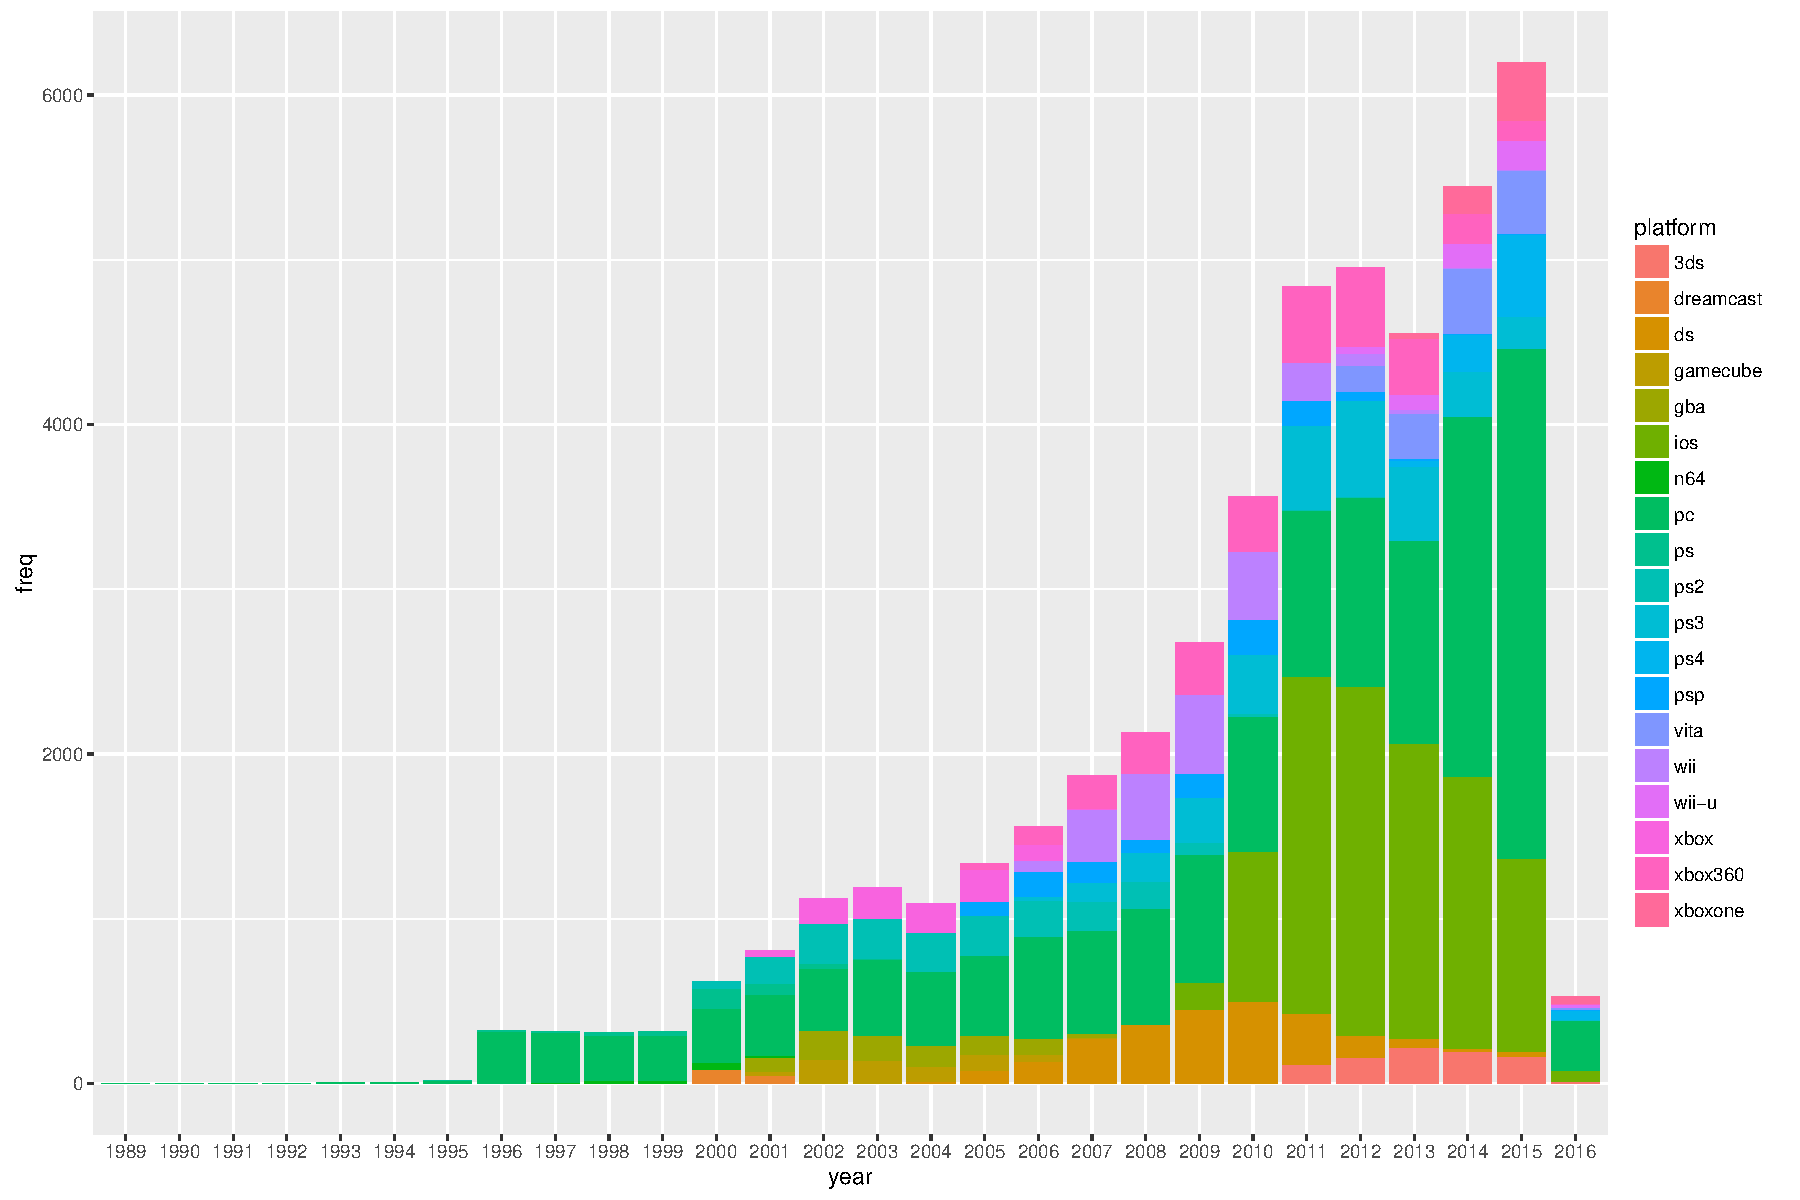
\includegraphics[width=1.0\columnwidth]{images/releases-per-year.pdf}
	\caption{Number of game releases per platform according to the Metacritic data.}
\label{fig:releases-per-year}
\end{figure}



%%%%%%%%%%%%
\subsubsection{platform-market-comparison/games-per-year.R}

 hat den ersten Versuch einer Nutzenrechnung für Spieler auf verschiedenen Plattformen. Script könnte leicht angepasst und erweitert werden. Beispielausgabe \ref{fig:gamesperyear-over-budget}, \ref{fig:steam-prices}

\begin{figure}[!t]
	\centering
	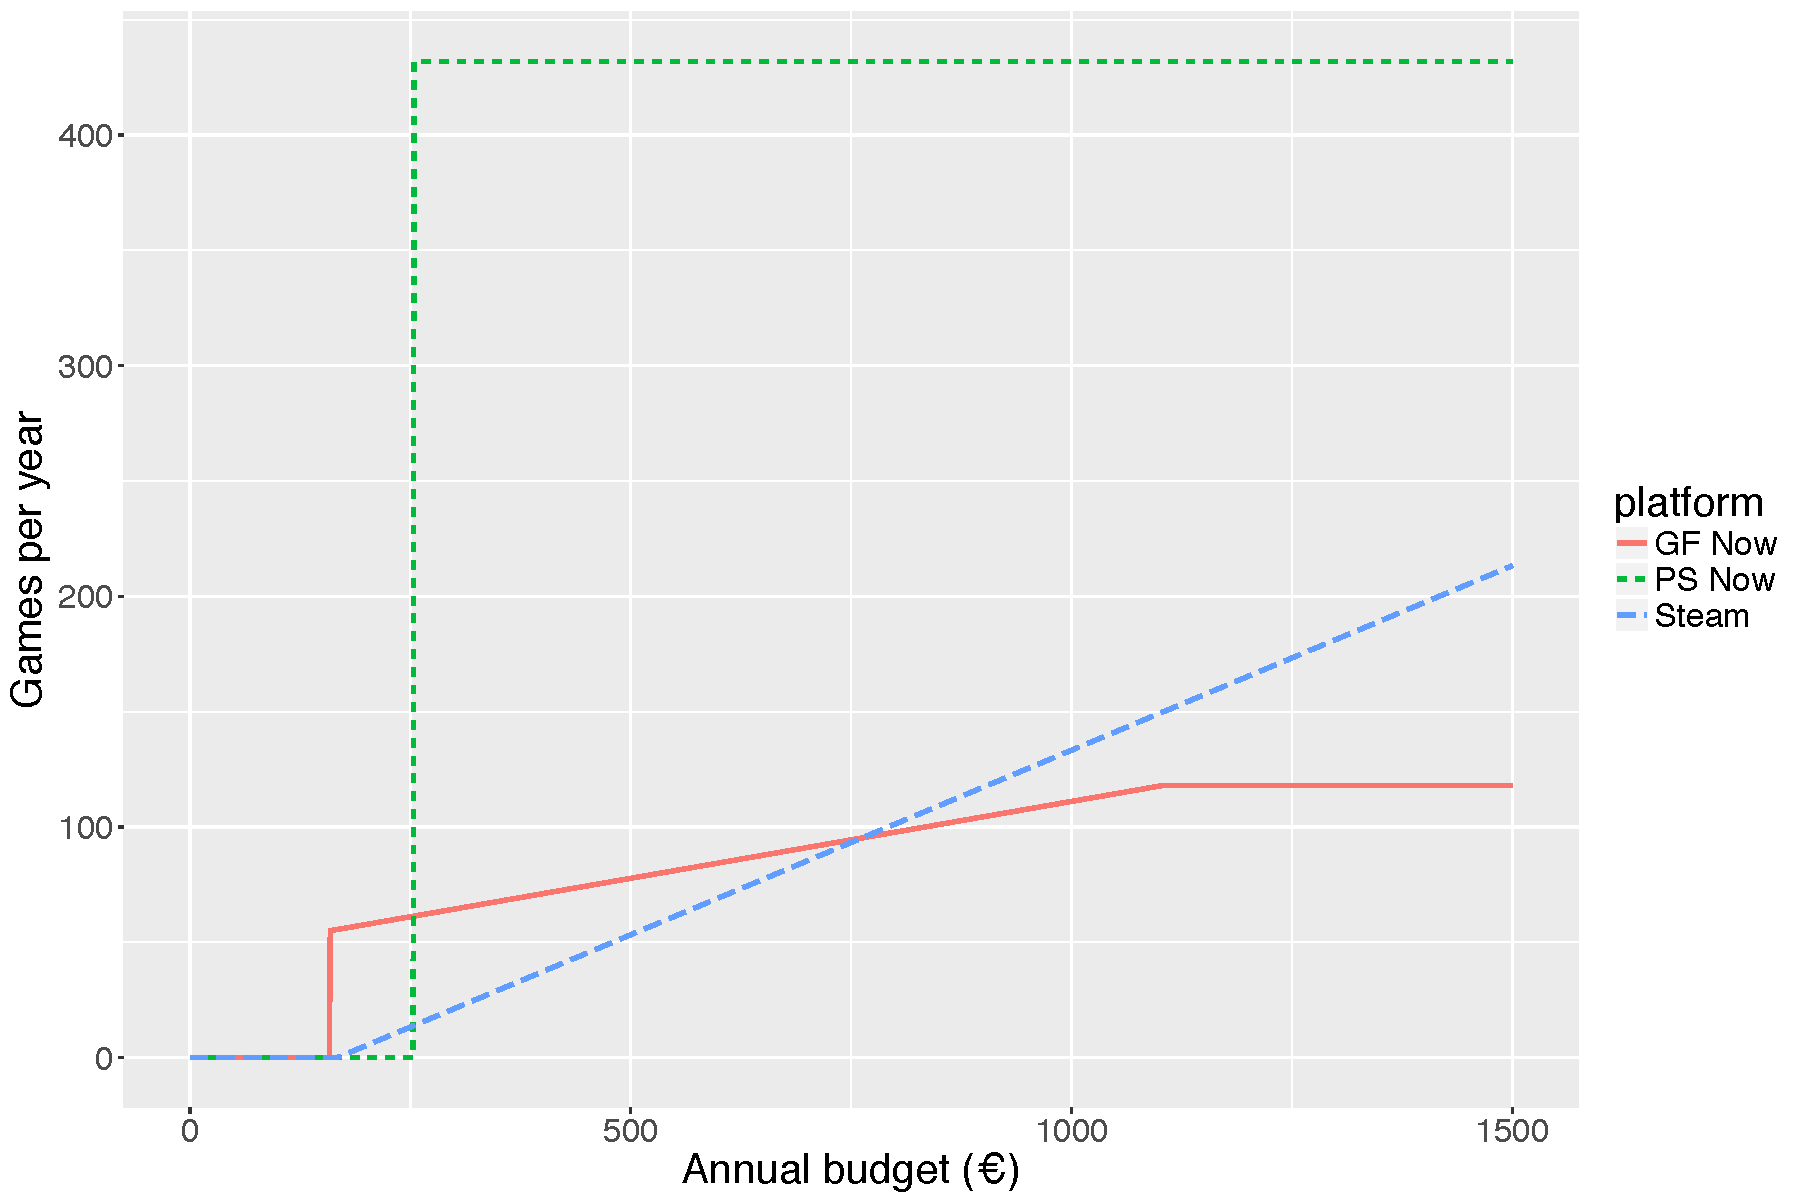
\includegraphics[width=1.0\columnwidth]{images/gamesperyear-over-budget.pdf}
	\caption{Models for several platforms showing the number of games per year that can be bought with a specific \$ budget.}
\label{fig:gamesperyear-over-budget}
\end{figure}

\begin{figure}[!t]
	\centering
	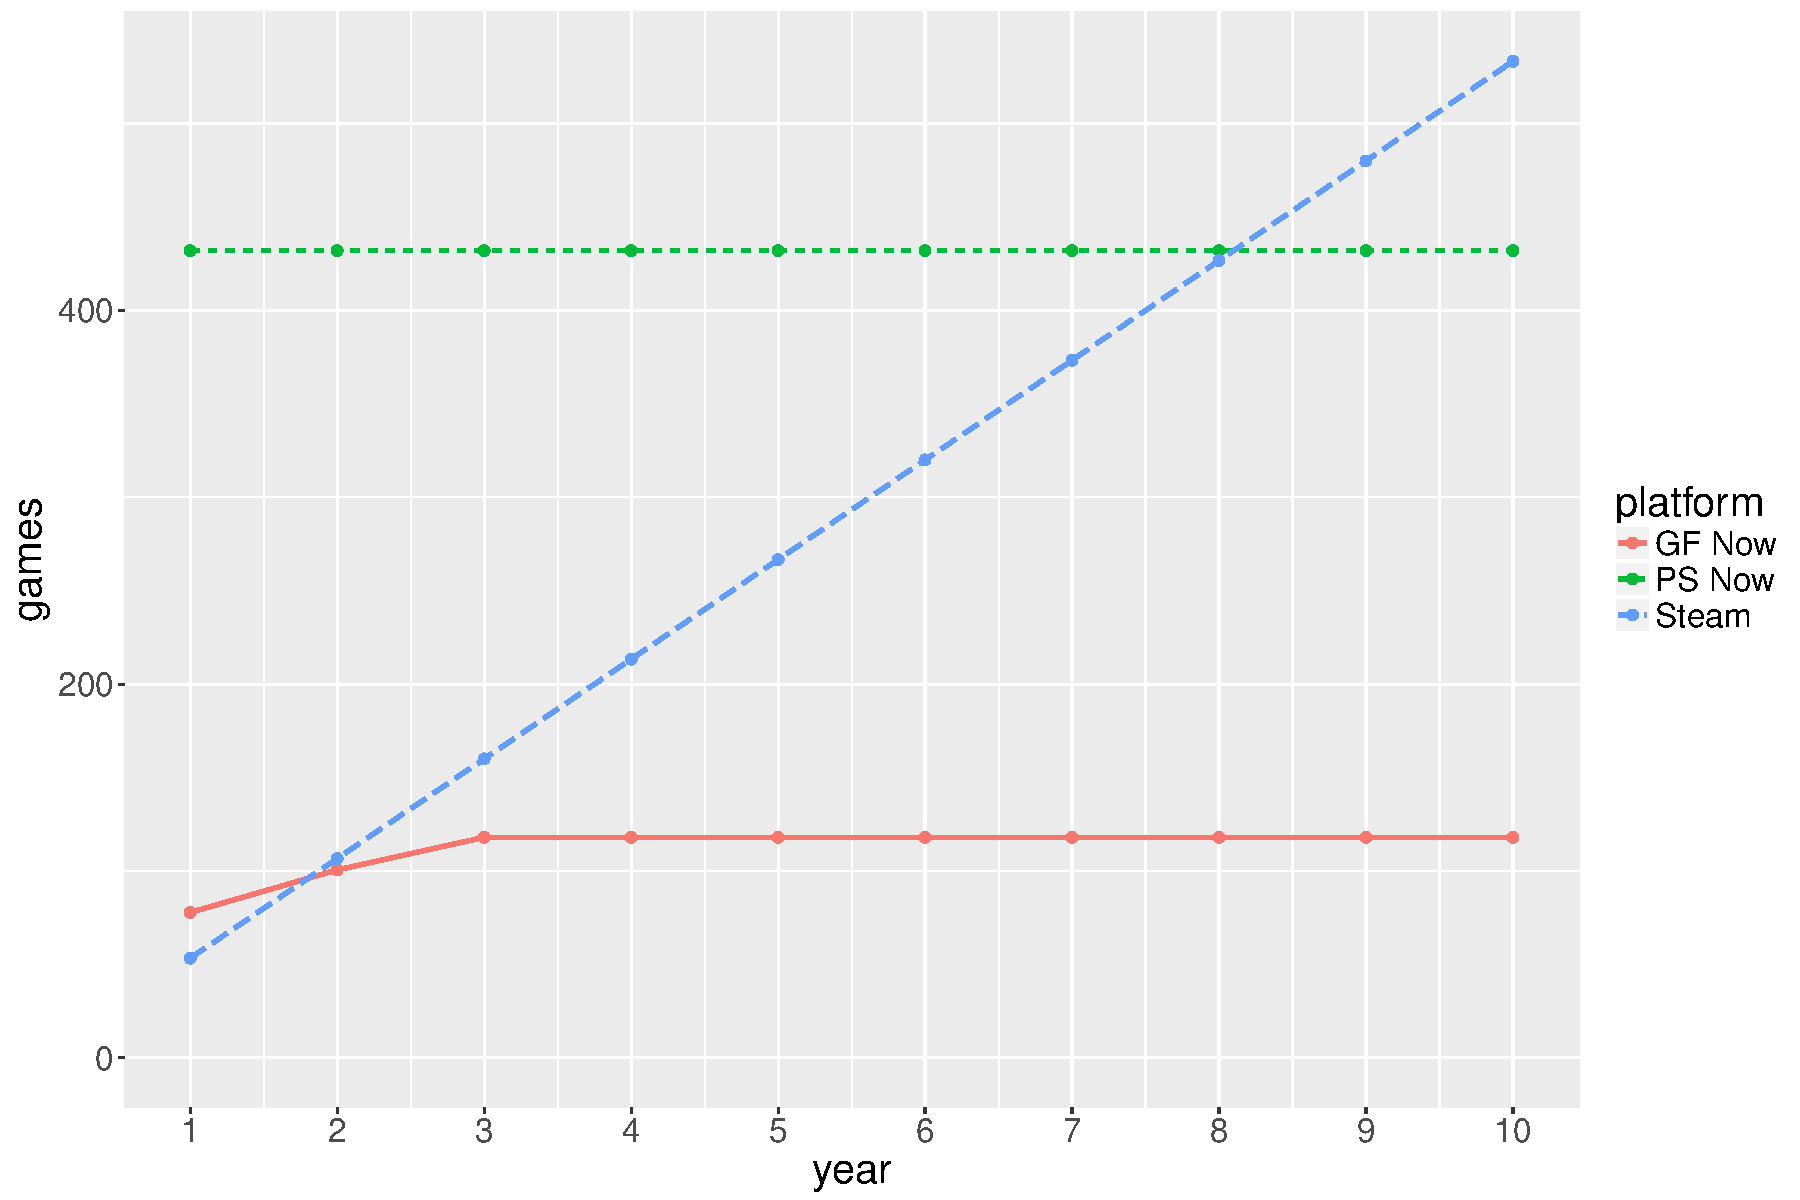
\includegraphics[width=1.0\columnwidth]{images/games-over-year.pdf}
	\caption{Models for several platforms showing the number of games that can be bought over the years subscribed to / using this service.}
\label{fig:games-over-years}
\end{figure}


\subsubsection{E2E Lag}
End-to-End Lag Model and Simulation in R. Now a standalone (submitted) paper at \url{https://github.com/mas-ude/onlinegame-lag-sim}. Can be referenced to argue the need for low E2E lag (meaning low network delay, but also the need for high fps).


%%%%%%%%%%%%
\subsubsection{Other Useful Data for Model Creation}

\begin{itemize}
	\item Game costs (current cost possible via Steam dataset; historic price data more difficult)
	\item Length of games (either via howlongtobeat dataset (via \url{https://github.com/mas-ude/gamelengths-scraper}), SteamSpy data, or could also additionally manually parse more Steam data)
	\item Gaming score/ratings/rankings (via Metacritic dataset (via \url{https://github.com/mas-ude/metacritic_scraper}), or might want to additionally scrape steam user review scores)
	\item Other popularity measures? (e.g. steamspy owner data?)
	\item Influence of E2E lag on games? (could be theorized indirectly through e2e lag sim + categorization attempts)
	\item Hardware requirements of games?

	\item Price History? Maybe using steamdb.info?
\end{itemize}


%!TEX root = paper.tex
%%%%%%%%%%%%%%%%%%%%%%%%%%%%%%%%%%%%%%%%%%%%%%%%%%%%%%%%%%%%%%%%%%%%%%%%%%%%%%%%
\section{Evaluation}
\label{sec:eval}

This section investigates the properties of the actual games offered on the
various platforms, so as to provide a backdrop against which utility
metrics can be viewed.
Table~\ref{tab:game-stats} provides an overview of the data.

\todo[inline]{Umsortieren um mit Background kohärent zu sein?}


% %!TEX root = paper.tex

\begin{table}
\caption{Metadata for the \steam, \metacritic, \hltb, \psnow, and \gfnow datasets. Records with a * note include games from other platforms than PC, PlayStation, and GeForce Shield.}
\label{tab:dataset-metadata}
\centering
\begin{tabu}{X[1.5]|X[r]|X[0.7,r]|X}
\toprule
Product & Date generated & \# of records & Method of generation\\
\midrule
\steam & 2015-07-14 & \num{5996} & Steam \& SteamSpy\\
\steam & 2015-10-30 & \num{6769} & Steam \& SteamSpy\\
\steam & 2016-02-06 & \num{7749} & Steam \& SteamSpy\\
\psnow & 2016-02-09 & \num{190} & Official list\\
\gfnow & 2016-02-12 & \num{69} & Manual screen scraping\\
\metacritic & 2016-03-02 & * \num{46197} & Web scraping\\
\hltb & 2016-03-01 & * \num{18433} & Web scraping\\
\bottomrule
\end{tabu}
\end{table}

% %!TEX root = paper.tex

\begin{table*}
\centering
\caption{Overview of datasets. Values with * are 99th percentiles chosen due to unrealistically large outliers.}
\label{tab:dataset-stats}
\begin{tabular}{c|c|r|r|r|r|r|r}
Dataset & Metric & Mean & Min & 1Q & Median & 3Q & Max\\
\hline
\hline
\steam & Number of records & \num{7749} & -- & -- & -- & -- & -- \\
\steam & Owners & \num{218112} & \num{0} & \num{4831} & \num{21740} & \num{107299} & \num{58666968} \\
\steam & players 2weeks & \num{9064} & \num{0} & \num{0} & \num{509} & \num{1526} & \num{7860554} \\
\steam & players forever & \num{138322} & \num{0} & \num{1780} & \num{9408} & \num{51997} & \num{58666968} \\
\steam & Average playtime (forever) & \num{507} & \num{0} & \num{93} & \num{200} & \num{429} & \num{45540} \\
\steam & Median playtime (forever) & \num{246} & \num{0} & \num{36} & \num{101} & \num{216} & \num{67538} \\
\steam & average 2weeks & \num{144} & \num{0} & \num{0} & \num{48} & \num{173} & \num{11387} \\
\steam & median 2weeks & \num{126} & \num{0} & \num{0} & \num{35} & \num{128} & \num{11387} \\
\steam & Price & \num{564} & \num{-1.26} & \num{0.99} & \num{3.39} & \num{7.49} & \num{119.00} \\
\hline
\psnow & Number of records & \num{252} & -- & -- & -- & -- & -- \\
\psnow & Rental fee for 4 hours & \num{3.02} & \num{1.99} & \num{1.99} & \num{2.99} & \num{2.99} & \num{22.99} \\
\psnow & Rental fee for 7 days & \num{5.48} & \num{1.99} & \num{3.99} & \num{4.99} & \num{5.99} & \num{14.99} \\
\psnow & Rental fee for 30 days & \num{8.40} & \num{3.99} & \num{5.99} & \num{6.99} & \num{7.99} & \num{22.99} \\
\psnow & Rental fee for 90 days & \num{12.57} & \num{3.99} & \num{7.99} & \num{8.99} & \num{14.99} & \num{49.99} \\
\hline
\gfnow & Number of records & \num{68} & -- & -- & -- & -- & -- \\
\gfnow & Price & \num{6.98} & \num{0} & \num{0} & \num{0} & \num{13.99} & \num{59.99} \\
\hline
\metacritic & Number of records & \num{45803} & -- & -- & -- & -- & -- \\
\metacritic & User score & \num{6.9} & \num{0} & \num{6.2} & \num{7.3} & \num{8.1} & \num{9.3} \\
\metacritic & Score & \num{69} & \num{8} & \num{62} & \num{72} & \num{79} & \num{96} \\
\hline
\hltb & Number of records & \num{18129} & -- & -- & -- & -- & -- \\
\hltb & Main story length & \num{26} & \num{0.02} & \num{2.5} & \num{6} & \num{12} & * \num{94} \\
\hltb & Main extra length & \num{21} & \num{0.08} & \num{5} & \num{10} & \num{20} & * \num{126} \\
\hltb & Completionist length & \num{28} & \num{0.03} & \num{5} & \num{13} & \num{29} & * \num{250} \\
\hltb & Combined length & \num{13} & \num{0.02} & \num{3} & \num{8} & \num{15} & \num{420} \\
\end{tabular}
\end{table*}

\todo[inline]{PZ: Viele daten, aber welche plattform ist die beste?}


%%%%%%%%%%%%

\begin{table*}
\centering
\caption{Game characteristics on the investigated platforms. Title counts from Web/API scraping, lengths from \hltb, ages and review scores from \metacritic.}
\label{tab:game-stats}
	\begin{tabu}{X[2]|X[r]X[r]X[r]X[r]X[r]X[r]X[r]}
	\toprule
	Service & Titles & Age $\mu$ & Age $\sigma$ & Length $\mu$ & Length $\sigma$ & Score $\mu$ & Score $\sigma$ \\
	\midrule
	\gfnow & $118$ & \SI{3.1}{\year} & \SI{\pm2.3}{\year} & \SI{10.7}{\hour} & \SI{\pm8.2}{\hour} & $73.9$ & $\pm10.1$ \\
	\psnow & $432$ & \SI{4.8}{\year} & \SI{\pm2.4}{\year} & \SI{8.8}{\hour} & \SI{\pm8.8}{\hour} & $71.9$ & $\pm12.0$ \\
	\steam & $14,120$ & \SI{2.5}{\year} & \SI{\pm3.3}{\year} & \SI{7.3}{\hour} & \SI{\pm10.2}{\hour} & $70.6$ & $\pm11.0$ \\
	\bottomrule
	\end{tabu}
\end{table*}


%%%%%%%%%%%%
\subsubsection{Number of Games}

The two cloud
platforms offer a very limited number of games when compared to the
games available on \steam, which itself again only represents a subset
of all games available either on the PC platform (\metacritic lists
$26,420$) or across all platforms ($57,308$ listed on the site). Two
possible, simple explanations for the low game count on the cloud
platforms come to mind: One is that they were launched relatively
recently (2015) in comparison to \steam (2003), leaving little time for
the range of games to grow. Secondly, the choice of games for a cloud
gaming platform is most likely curated by the platform operator for
compatibility and performance reasons. This usability burden shifts to
the end user for digital storefronts like \steam, allowing these
platforms to offer a larger variety of games, including ones that are
very demanding on the hardware. Furthermore, the business models
of the \gls{cg} platforms are still in flux, as described earlier.


%%%%%%%%%%%%
\subsubsection{Game Ages}

Game ages appear to be relatively high for all of the investigated
platforms, and particularly so for \psnow. It might be considered a
special case, as it is specifically advertised as a backwards
compatibility for older, pre-PlayStation 4 games that do not run on the
latest Sony platform any more. For \steam, the distribution is
significantly skewed towards recent titles: A quarter of games are less
than $10$ months old, and the median is at $21$ months. The
distribution's tail extends well beyond $25$ years (due to re-releases
of ``classic'' games on the platform).


%%%%%%%%%%%%
\subsubsection{Game Lengths}
Figure~\ref{fig:gamelengths-violin} shows the distribution of aggregated
game lengths for the three platforms under investigation, and an
``overall'' distribution that includes further platforms and gaming
systems. Among the three platforms, the mean and median reported game
lengths (approximately \SI{14}{\hour}) are largest for \gfnow. In
contrast to the curated choice of games on the Cloud systems, \steam
also offers shorter and longer games.


\begin{figure}[!t]
	\centering
	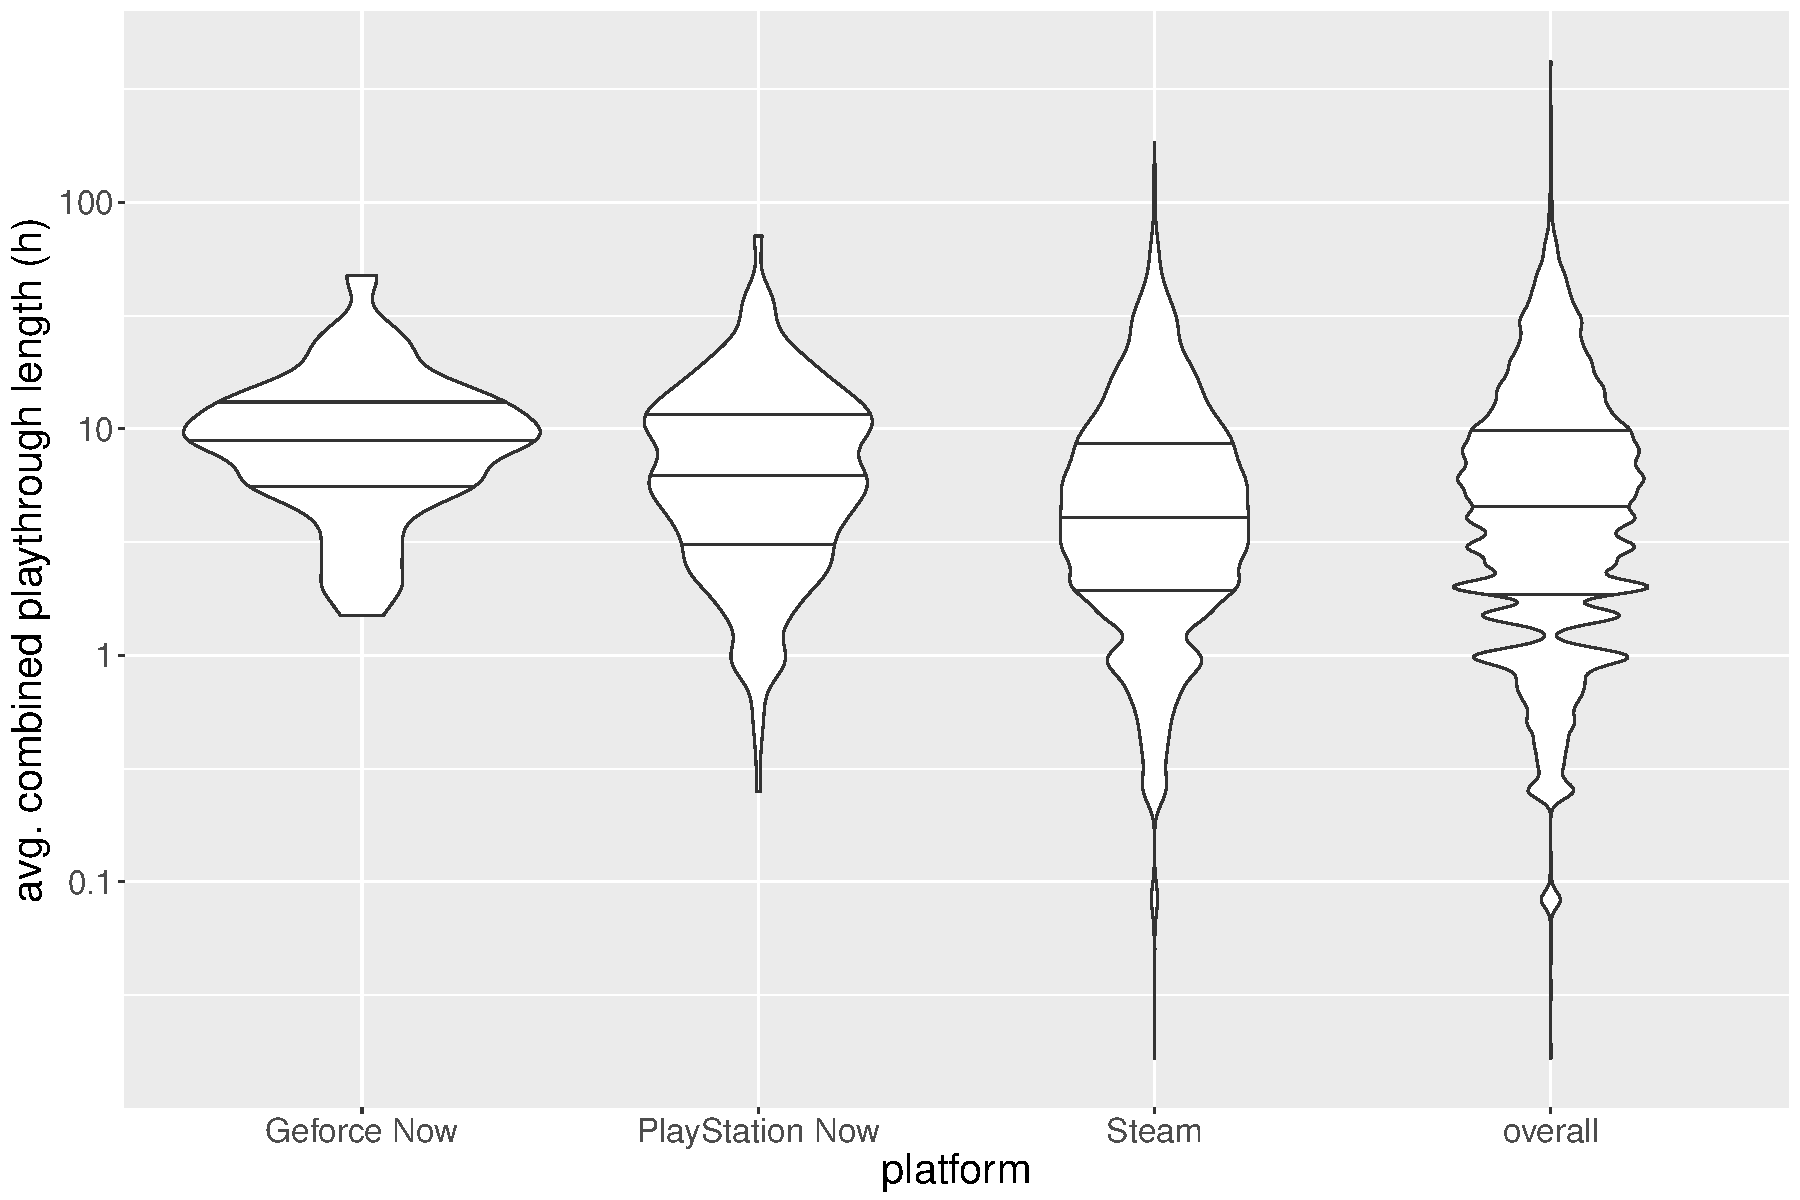
\includegraphics[width=1.0\columnwidth]{images/gamelengths-by-platform-violin.pdf}
	\caption{Violin plot of the per-platform average game lengths from \hltb. Quartiles indicated by horizontal lines.}
%	aggregated over all play styles (raw data source: \hltb).}
\label{fig:gamelengths-violin}
\end{figure}



%%%%%%%%%%%%
\subsubsection{Game Prices}

Trying to compare the prices per game is a difficult endeavor, due to
the mixed approach of the gaming platforms. The \gfnow subscription
gives customers access to a subset of its catalog that can be
extended by purchasing additional games; \gfnowpc and \liquid
on the other hand require the customer to buy games on their
own and pay for the
time spent playing.
\psnow and \psnowpc have a flat rate for all of their catalog.
%Furthermore, the exact subscription and rental modalities as well as prices are adapted over time, and differ between regional markets.
%\todo[inline]{SV:The last sentence was somehow superfluous since variety over time is the case for all of our data. --> erased it.}
At least for \steam, unit prices can be discussed.

\begin{table}
\centering
\caption{Overview of average prices and counts for \steam games.}
\label{tab:steam-price-stats}
\begin{tabu}{X[2]|X[r]X[r]X[r]X[r]X[r]X[r]X[r]X[r]}
	\toprule
	\textbf{Date} & 2015-07 & 2015-10 & 2016-02 & 2016-06 & 2016-09 & 2016-11 & 2017-04 & 2017-10 \\
	\midrule
	\textbf{Average price (€)} & $10.11$ & $8.47$ & $5.65$ & $4.72$ & $8.77$ & $5.33$ & $9.95$ & $8.83$ \\
	\midrule
	\textbf{Standard deviation (€)} & $\pm12.03$ & $\pm9.74$ & $\pm7.88$ & $\pm7.02$ & $\pm10.83$ & $\pm11.08$ & $\pm29.94$ & $\pm12.2$ \\
	\midrule
	\textbf{Number of games} & $5,996$ & $6,769$ & $7,749$ & $9,187$ & $10,191$ & $10,077$ & $11,612$ & $14,120$ \\
	\bottomrule
\end{tabu}
\end{table}


\begin{figure}[!t]
	\centering
	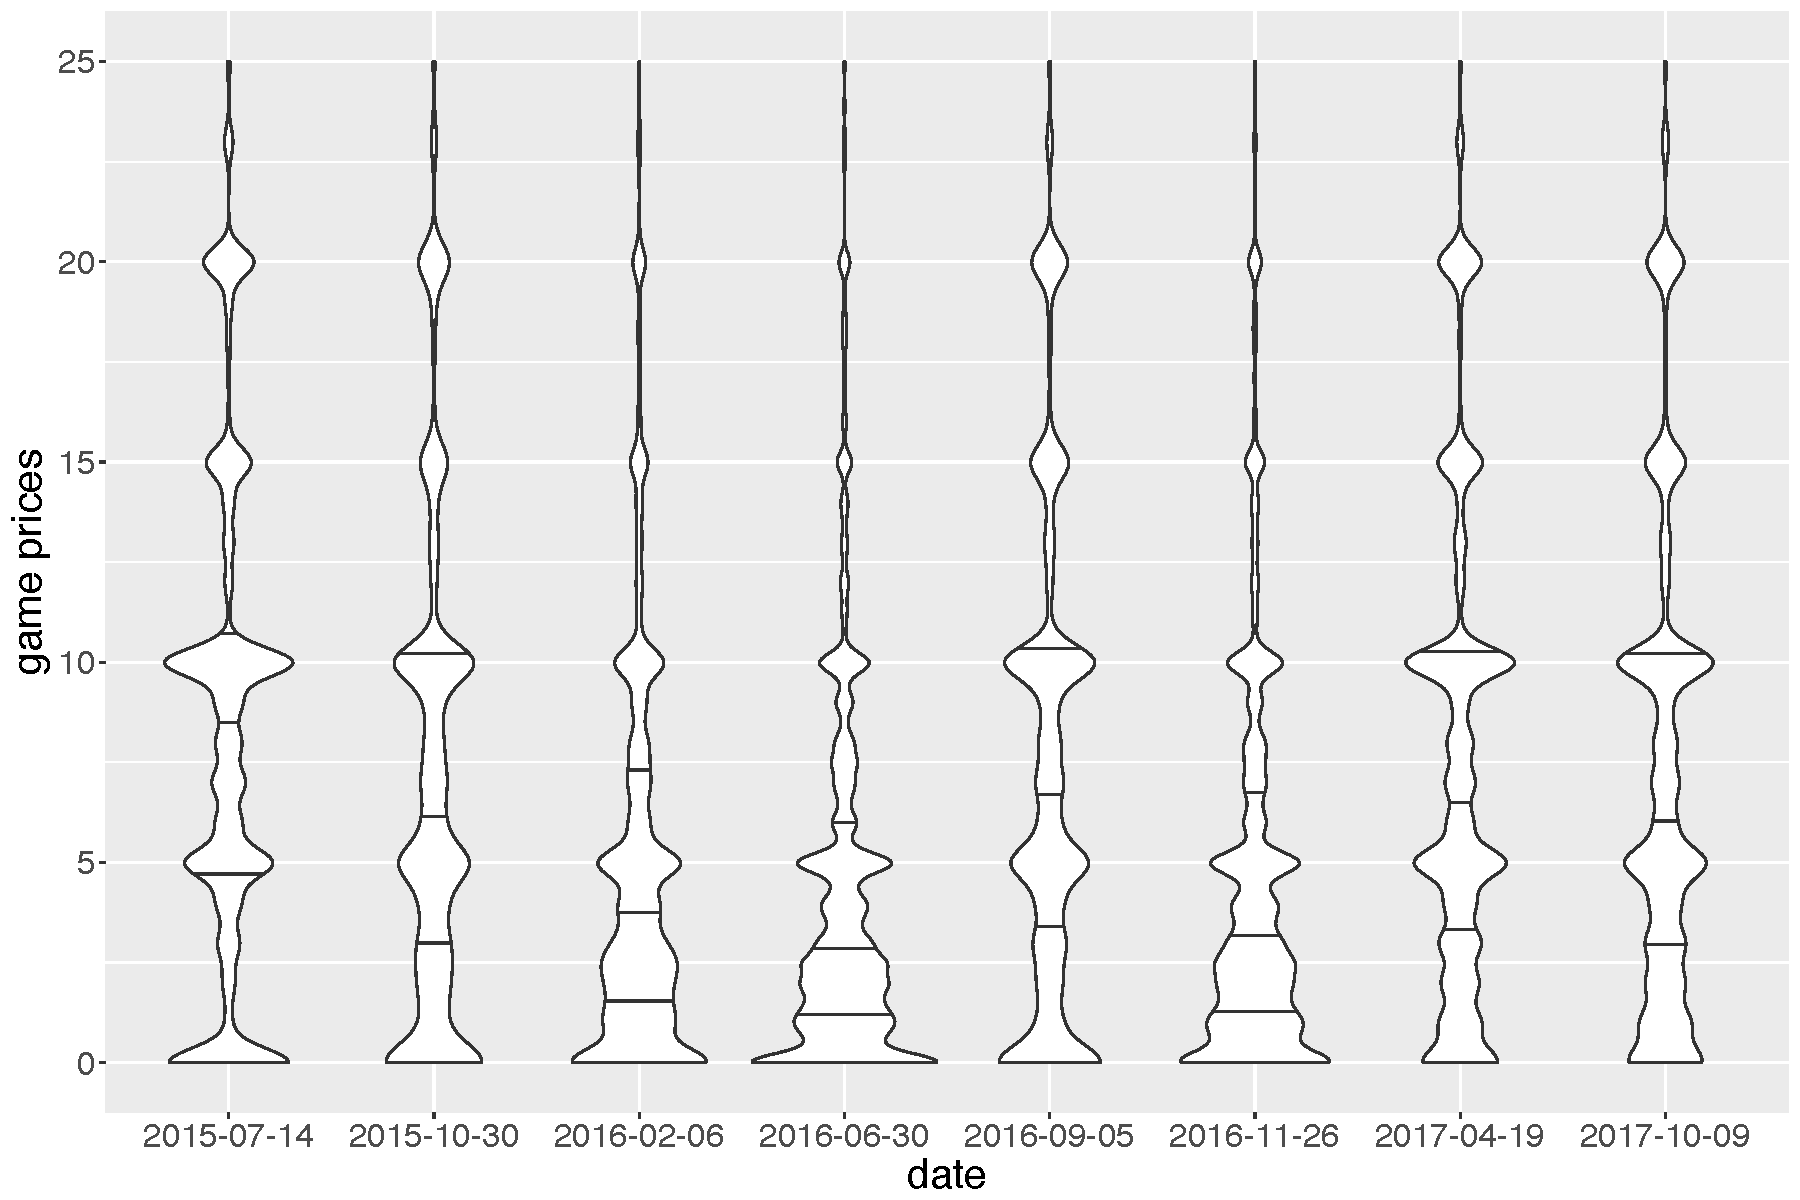
\includegraphics[width=1.0\columnwidth]{images/steam-price-violins-over-time.pdf}
	\caption{Violin plot of prices of \steam games over time. Quartiles indicated by horizontal lines.}
\label{fig:steam-price-violins}
\end{figure}
%# Some modes for 2017-10-09, see steam-prices.R
%#         10% of games are free
%# (18-13)= 5% of games cost  0.99
%# (30-26)= 4% of games cost  2.99
%# (48-36)=12% of games cost  4.99
%# (76-63)=13% of games cost  9.99
%# (87-82)= 5% of games cost 14.99
%# (93-89)= 4% of games cost 19.99
%# The top  6% of games cost more than that


Table~\ref{tab:steam-price-stats} shows the development of average
\steam game prices with standard deviations and the number of available
games for all \steam measurements taken so far, spanning a time interval
of more than two years. As can be seen, the number of games offered
has more than doubled since the first data point, while the average
prices fluctuate over time.
Figure~\ref{fig:steam-price-violins} complements the table, showing
smoothed density functions of the game price distributions in \steam's
store over time in the form of a violin plot.
Evidently, all distributions have modes (most prominently at nonegative
multiples of $\texteuro 5$), and exhibit strong temporal effects.
The variability can be explained by \steam's regular offer of sales
periods with reduced prices. For instance, the shift towards lower
prices in February 2016 coincides with a seasonal sales campaign
for Lunar New Year\footnote{\url{http://store.steampowered.com/news/20313/}}.

% Looking at the distributions of game prices, we find that the number of games in the sub \SI{5}]\EUR] category has ... hmm, what ... doubled? ... care to check with R?

%The influence of sales periods can be easily observed in the \acrshort{CDF} of prices in Fig. \ref{fig:steam-prices}, where the data from February was collected during \steam's Lunar New Year Sale.

%\begin{figure}[!t]
%	\centering
%	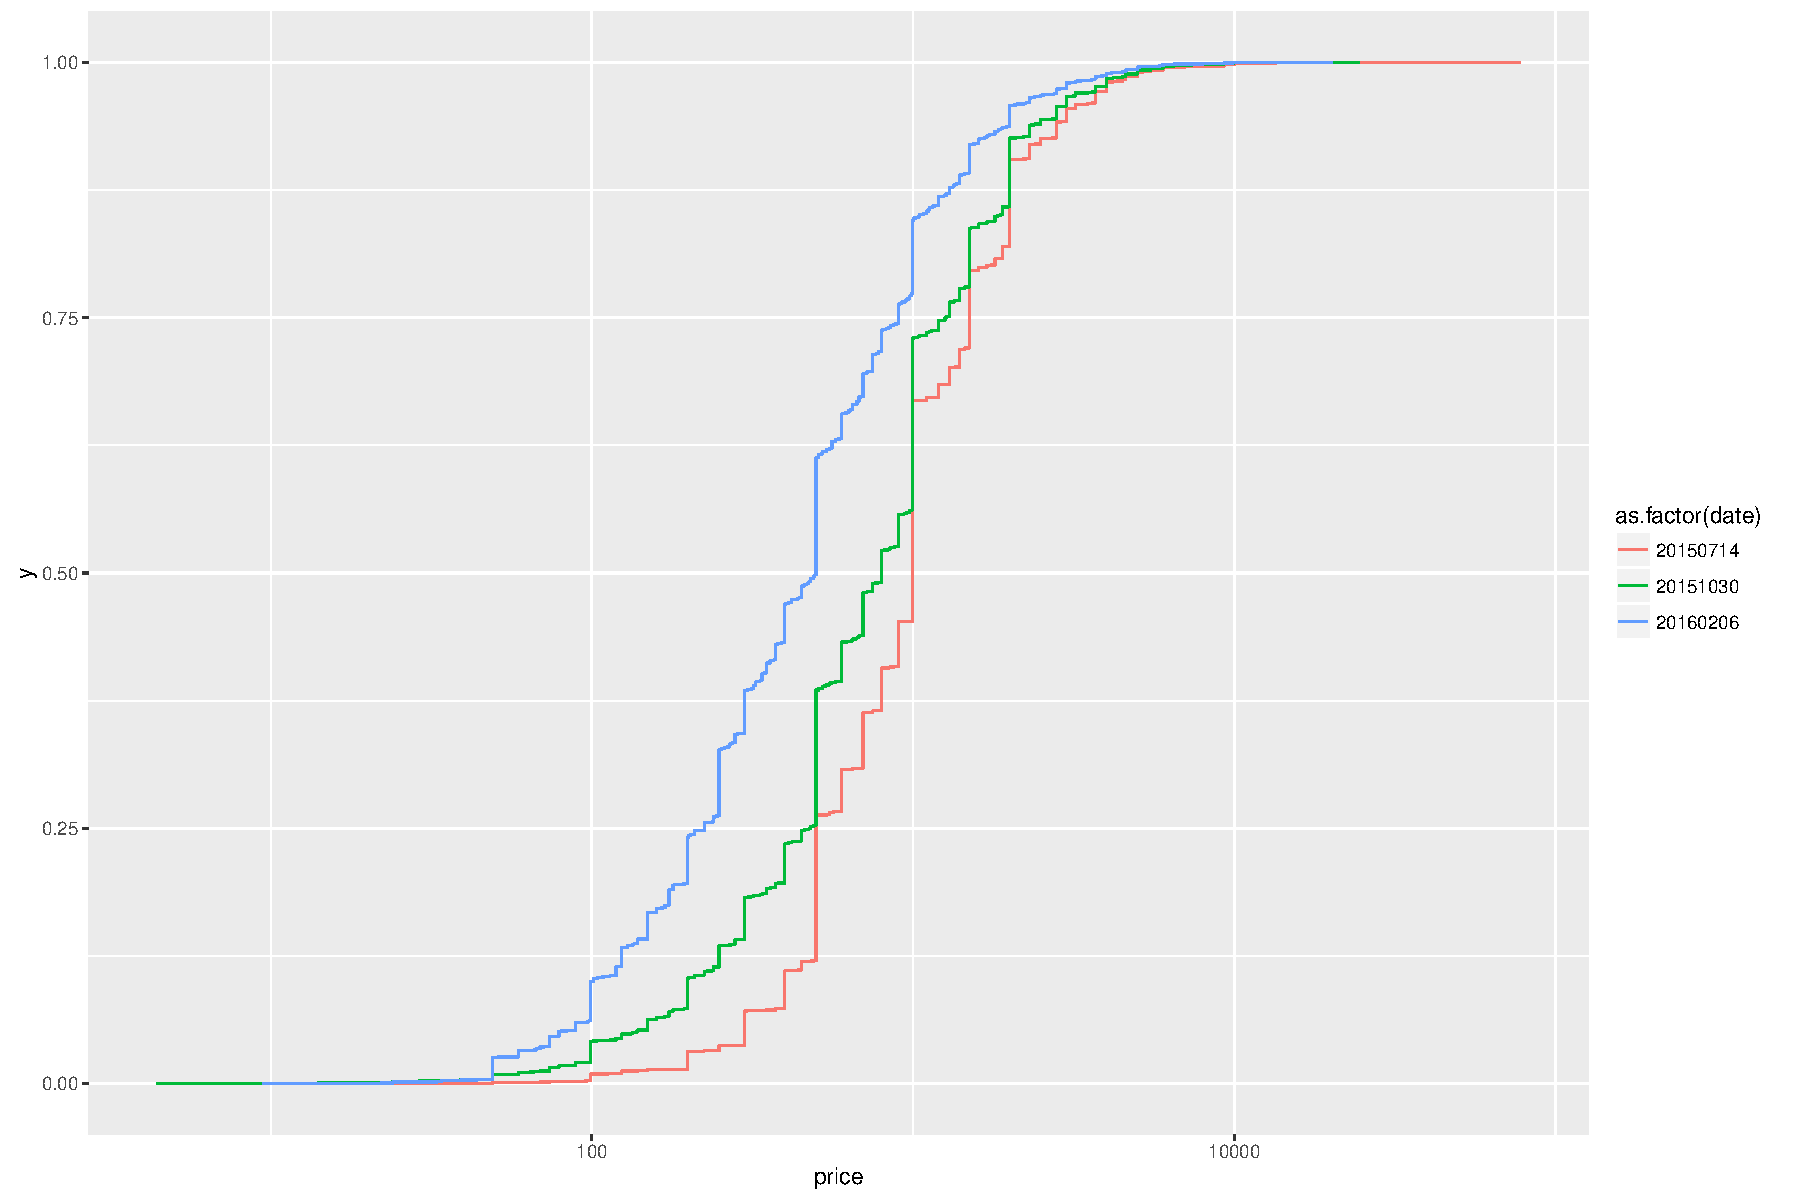
\includegraphics[width=1.0\columnwidth]{images/steam-prices.pdf}
%	\caption{CDF of games on the \steam platform at three distinct dates. The February data was collected in a sales period.}
%\label{fig:steam-prices}
%\end{figure}

\begin{figure}[!t]
	\centering
	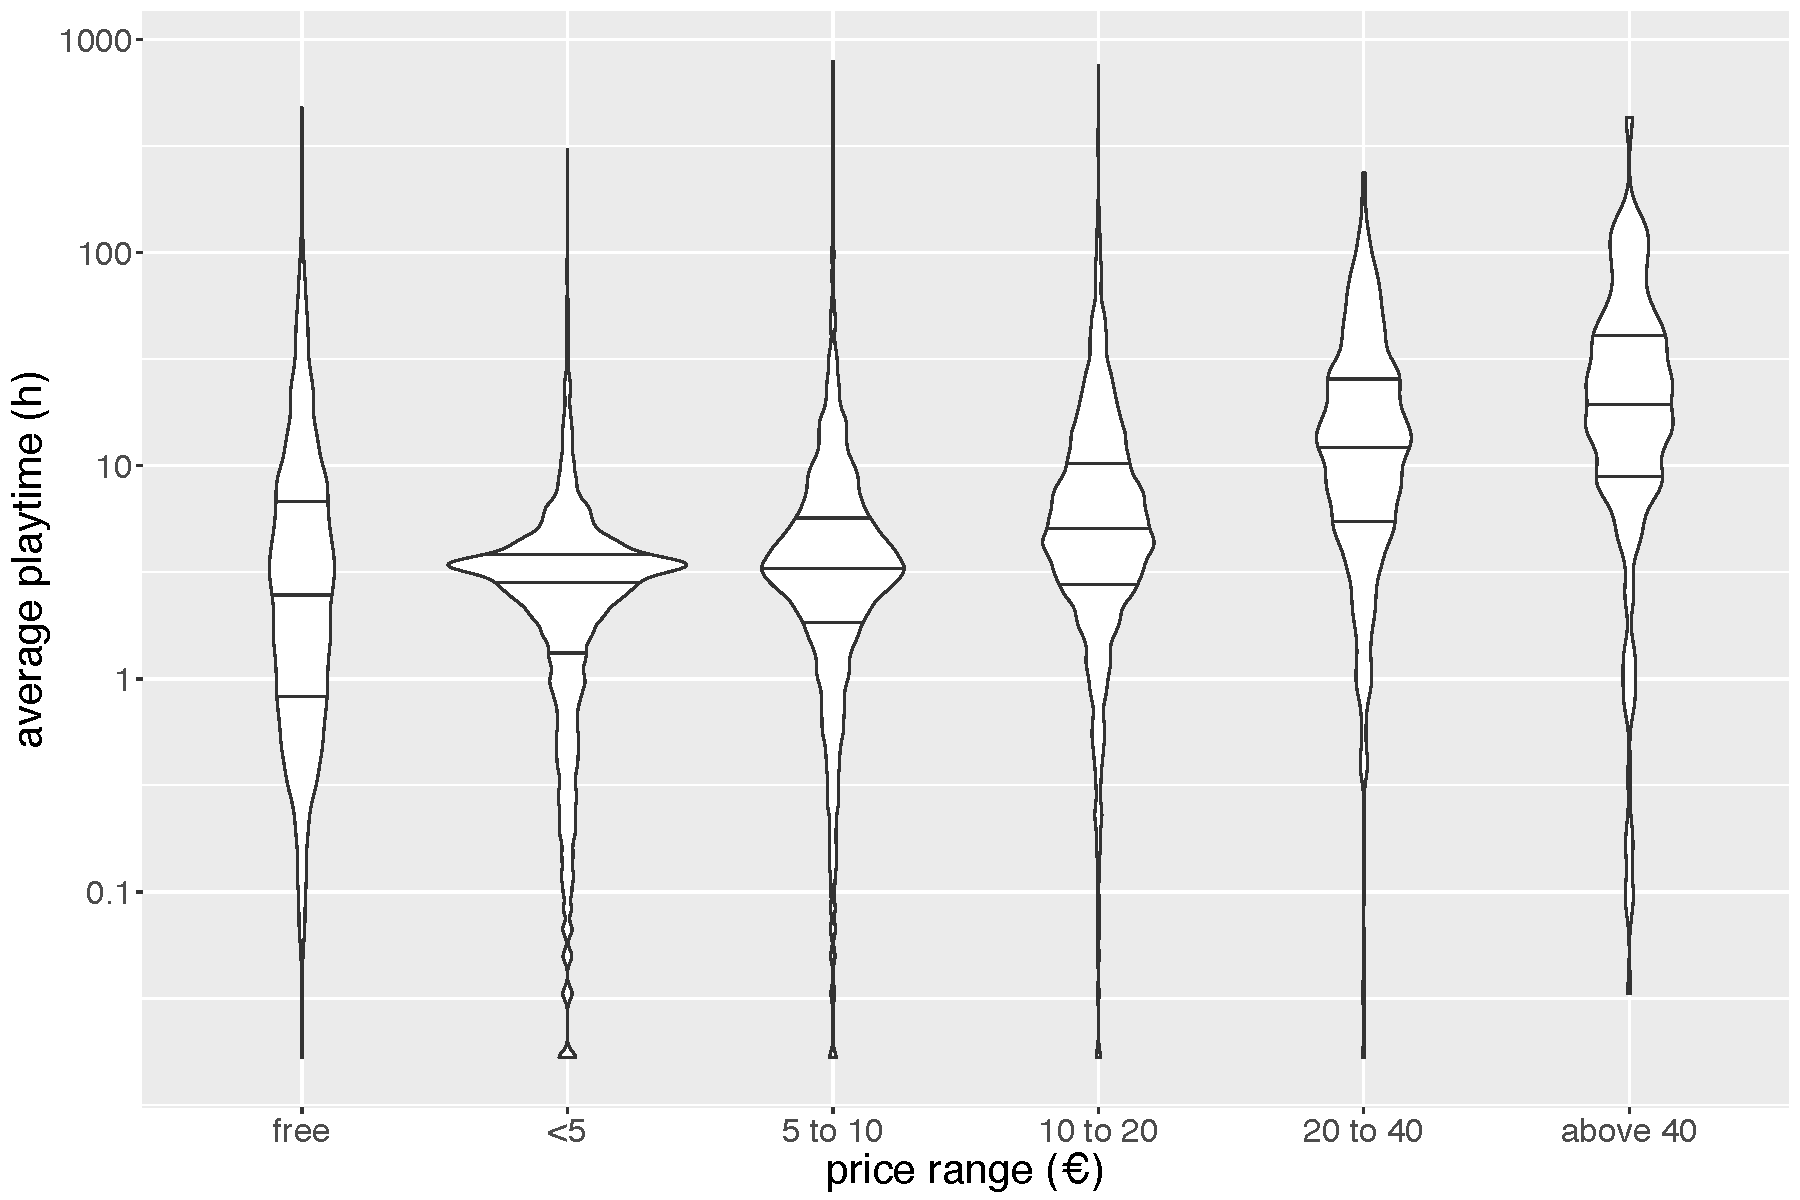
\includegraphics[width=1.0\columnwidth]{images/steam-cost-vs-playtime-non-sale.pdf}
	\caption{Violin plot of the average playtime of \steam games, broadly categorized by their price ranges. The number of games per bin are $1541$, $5269$, $4019$, $2445$, $658$, and $188$. Quartiles indicated by horizontal lines.}
\label{fig:steam-cost-vs-playtime-violin}
\end{figure}

\subsubsection{Price versus Playtime}
Again focusing on \steam,
Figure~\ref{fig:steam-cost-vs-playtime-violin} breaks down the
distribution of average playtimes per game price range. The game price
ranges are chosen so as to roughly separate the prevalent modes of the
price distribution.
Playtime is defined as the time game owners spend playing a game, as
recorded by the \steam platform and scraped from \textit{SteamSpy}.
On the far left in the Figure, playtimes of ``free'' titles
(including free-to-play games with monetization options other than an
upfront payment) span almost the whole playtime range with an
inter-quartile range of 45 minutes to about seven hours.
For games that cost less than $\texteuro 5$, the mode is around
3.5 hours of playtime, and values are concentrate around it. The
latter is of special interest because it is a recent trend that only
manifested itself in datasets in the last ten months. It seems that
game producers see this combination of price and playtime as a sweet
spot, as the number of games in this category grew by a factor of
2.4 in that timeframe --- for comparison, the number of games
increased by 37 percent in the free price range, and roughly doubled
in the other price ranges.

Other than that, the median playtime increases with the price range;
unfortunately, the data does not explain the cause: E.g., more expensive
games might have more playable content, causing the playtime to
increase. Conversely, higher upfront costs may incite players to spend
more time regardless of game quality, thus avoiding regret for the
expense.
% Svenja deleted the following sentence since that can be the case anywhere:
%And still alternatively, there might exist an outside, common reason causing both parameters to increases.
Due to the strong popularity of \steam in \gls{PC} gaming (even physical
retail copies often require using the service nowadays) this set also
gives a good overview of the dimensions of \gls{PC} gaming in general.


%%%%%%%%%%%%
\subsubsection{Review Scores}

The final characteristic in this analysis are game review scores as
given by professional gaming media outlets. This relies on the
\metacritic dataset again. This set covers review scores for all current
and historic gaming platforms. The review scores are aggregated to
average scores ranging between $0$ and $100$. Some \metacritic-internal
weighing factors are applied to express the importance of some media
outlets over others.
The average scores seem quite similar across all services, albeit with a
slightly lower $\sigma$ for \gfnow. Figure~\ref{fig:scores-by-platform}
shows the distribution of review scores per platform. Both Cloud
services seem to favor certain score levels. Specifically, their lowest
quartiles (representing the worst-rated games on these platforms) reach
much higher values than \steam's. This could be an effect of the Cloud
systems curating the game offer to focus on highly-rated (and thus
perhaps more attractive) titles. \steam on the other side is a more or
less open platform, where every game publisher can sell their games at
their own volition (platform operator collects a commission fee for
sales). Consequently, it is reasonable to assume more variation in the
quality of games, which could in turn lead to mixed reviews.
%Cloud gaming platforms have to acquire licenses from the individual games' publishers and therefore have to be selective and curated by nature.
%\todo[inline]{AR: Should we mention other possible effects such as ``Metacritic probably isn't free of bias (gosh!)''?}
% that would only lead to a very, very lengthy off-topic discussion, so probably no

% TODO: include or compare with data from opencritic.com as soon as their API is public/usable

% \begin{figure}[!t]
% 	\centering
% 	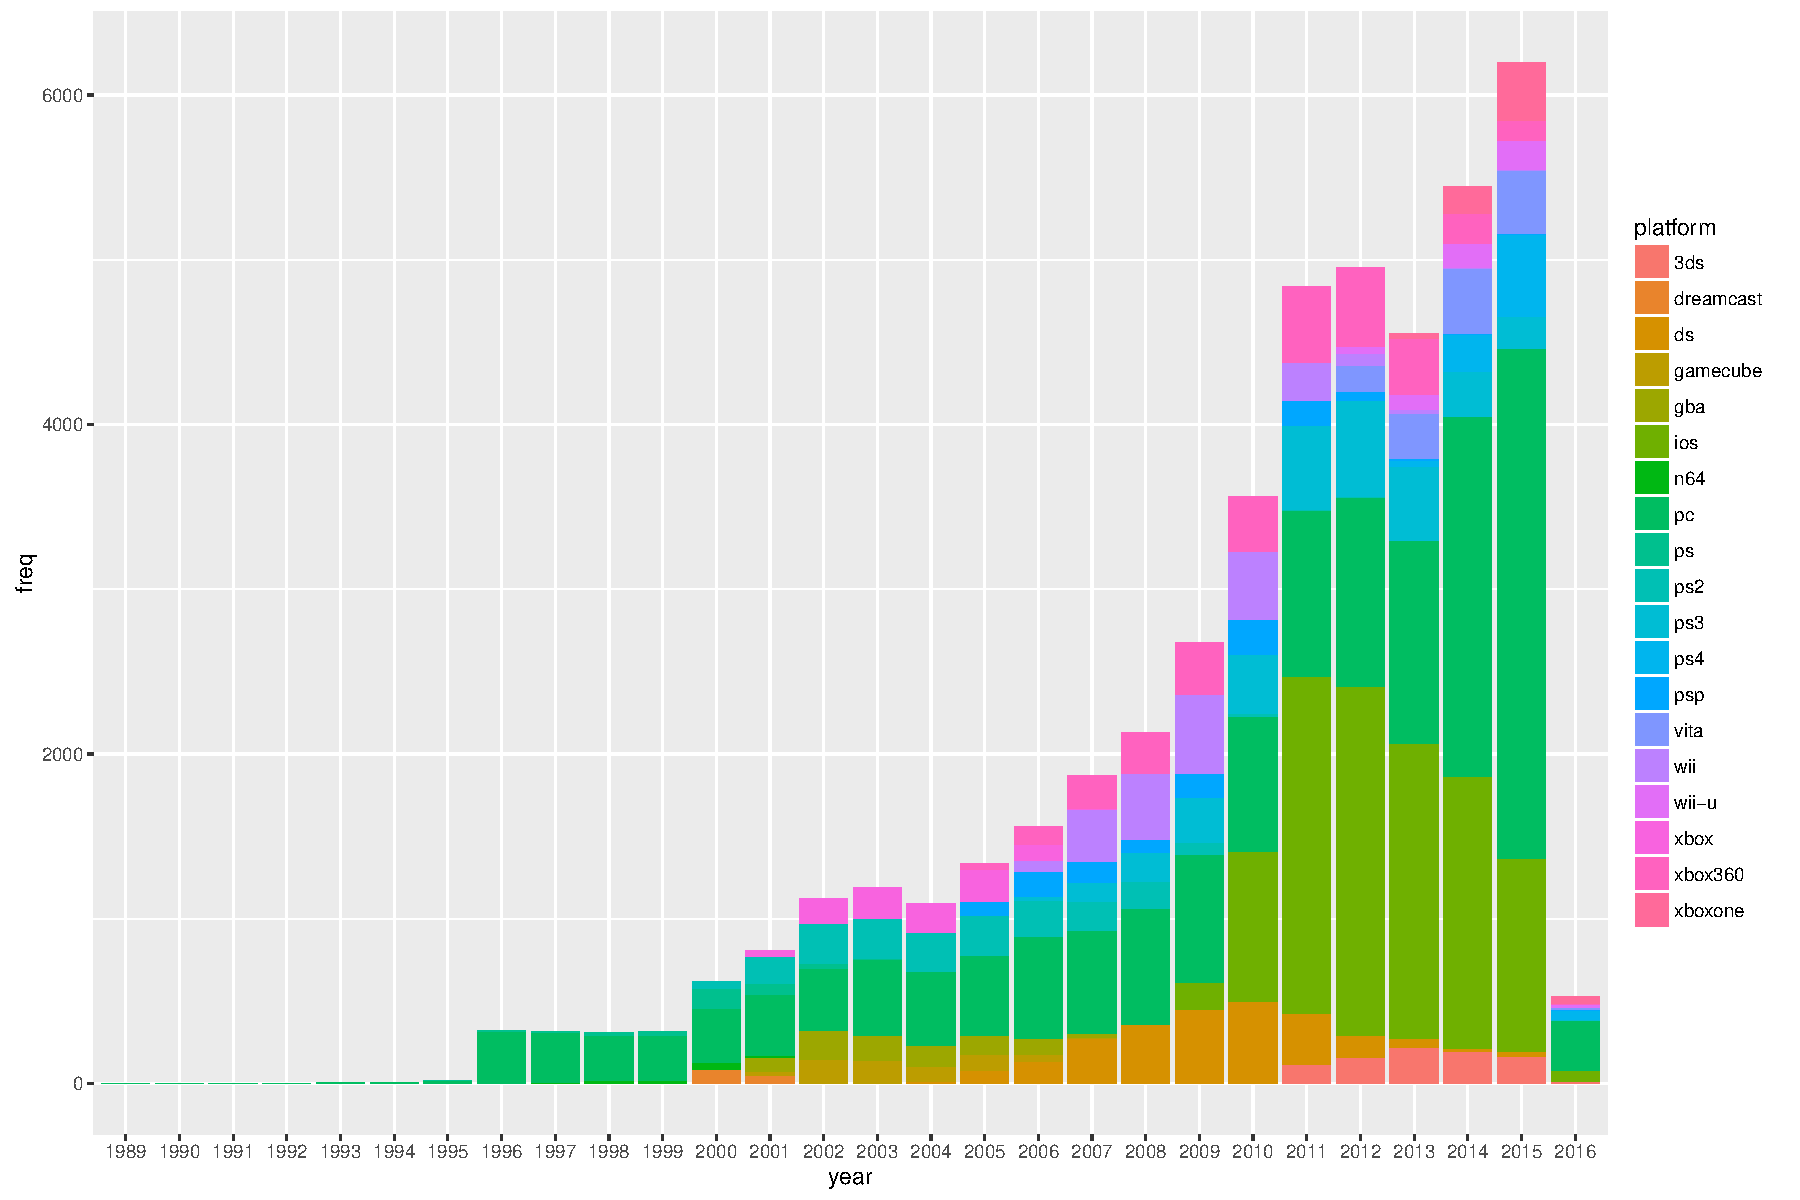
\includegraphics[width=1.0\columnwidth]{images/releases-per-year.pdf}
% 	\caption{Number of game releases per platform according to the Metacritic data.}
% \label{fig:releases-per-year}
% \end{figure}

\begin{figure}[!t]
	\centering
	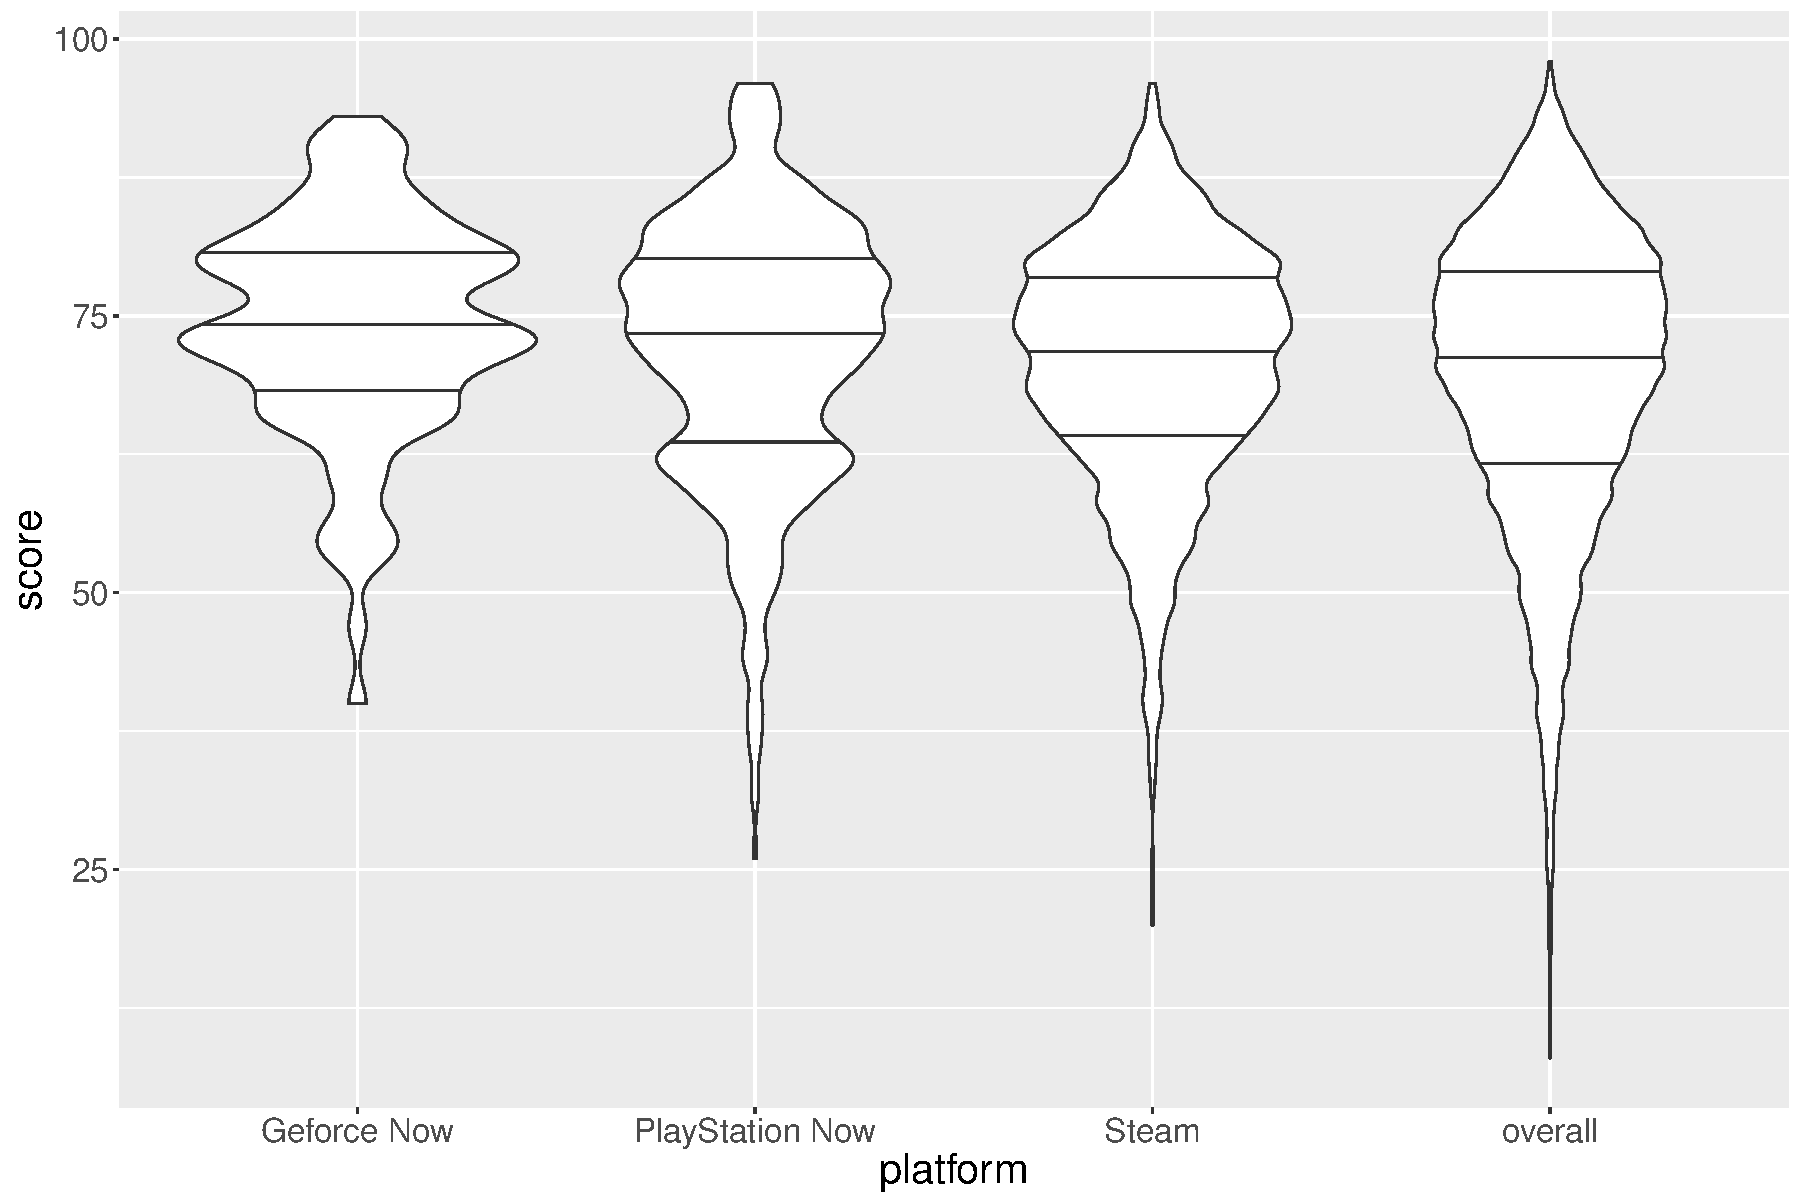
\includegraphics[width=1.0\columnwidth]{images/scores-by-platform-violin.pdf}
	\caption{Violin plot of aggregated review scores per platform. Quartiles indicated by horizontal lines.}
\label{fig:scores-by-platform}
\end{figure}


%!TEX root = paper.tex
%%%%%%%%%%%%%%%%%%%%%%%%%%%%%%%%%%%%%%%%%%%%%%%%%%%%%%%%%%%%%%%%%%%%%%%%%%%%%%%%
\section{Conclusion}
\label{sec:conclusion}

While cloud gaming is a topic of strong interest, it comes with a series of problems and limitations, both technical as well as economic in nature. With the conducted user-side analysis it is easy to see the different, curated nature of current cloud gaming services, with their narrow offer of hand-selected games, in the case of \psnow even catered to a specific audience. This limits the attractiveness of any such service, even without looking at more intricate engagement metrics which would require more data than what was available.

But also the operator-side reveals major problems due to the need for highly regional data-centers and special hardware. This eliminates any chance for the efficiency gains that general cloud services are intended for.

However, there might be some niches for specific games or audiences that could be sustained at reduced operational efforts. This might be an angle worth of investigation in the future, especially with better engagement metrics and more detailed models of gaming data center operations.

However, there might also be a simpler and economically more feasible alternative to cloud gaming: game streaming in the local network, which would combine the open market structures of conventional gaming platforms with the ease of use of having a small box in the living that one just can play games on without much thought to the underlying hardware.


\printbibliography

\balance

\end{document}
